% Options for packages loaded elsewhere
% Options for packages loaded elsewhere
\PassOptionsToPackage{unicode}{hyperref}
\PassOptionsToPackage{hyphens}{url}
\PassOptionsToPackage{dvipsnames,svgnames,x11names}{xcolor}
%
\documentclass[
  10pt,
  a4paper,
  DIV=11,
  numbers=noendperiod]{scrartcl}
\usepackage{xcolor}
\usepackage[top=22mm,bottom=22mm,left=22mm,right=22mm]{geometry}
\usepackage{amsmath,amssymb}
\setcounter{secnumdepth}{-\maxdimen} % remove section numbering
\usepackage{iftex}
\ifPDFTeX
  \usepackage[T1]{fontenc}
  \usepackage[utf8]{inputenc}
  \usepackage{textcomp} % provide euro and other symbols
\else % if luatex or xetex
  \usepackage{unicode-math} % this also loads fontspec
  \defaultfontfeatures{Scale=MatchLowercase}
  \defaultfontfeatures[\rmfamily]{Ligatures=TeX,Scale=1}
\fi
\usepackage{lmodern}
\ifPDFTeX\else
  % xetex/luatex font selection
\fi
% Use upquote if available, for straight quotes in verbatim environments
\IfFileExists{upquote.sty}{\usepackage{upquote}}{}
\IfFileExists{microtype.sty}{% use microtype if available
  \usepackage[]{microtype}
  \UseMicrotypeSet[protrusion]{basicmath} % disable protrusion for tt fonts
}{}
\usepackage{setspace}
\makeatletter
\@ifundefined{KOMAClassName}{% if non-KOMA class
  \IfFileExists{parskip.sty}{%
    \usepackage{parskip}
  }{% else
    \setlength{\parindent}{0pt}
    \setlength{\parskip}{6pt plus 2pt minus 1pt}}
}{% if KOMA class
  \KOMAoptions{parskip=half}}
\makeatother
% Make \paragraph and \subparagraph free-standing
\makeatletter
\ifx\paragraph\undefined\else
  \let\oldparagraph\paragraph
  \renewcommand{\paragraph}{
    \@ifstar
      \xxxParagraphStar
      \xxxParagraphNoStar
  }
  \newcommand{\xxxParagraphStar}[1]{\oldparagraph*{#1}\mbox{}}
  \newcommand{\xxxParagraphNoStar}[1]{\oldparagraph{#1}\mbox{}}
\fi
\ifx\subparagraph\undefined\else
  \let\oldsubparagraph\subparagraph
  \renewcommand{\subparagraph}{
    \@ifstar
      \xxxSubParagraphStar
      \xxxSubParagraphNoStar
  }
  \newcommand{\xxxSubParagraphStar}[1]{\oldsubparagraph*{#1}\mbox{}}
  \newcommand{\xxxSubParagraphNoStar}[1]{\oldsubparagraph{#1}\mbox{}}
\fi
\makeatother


\usepackage{longtable,booktabs,array}
\newcounter{none} % for unnumbered tables
\usepackage{calc} % for calculating minipage widths
% Correct order of tables after \paragraph or \subparagraph
\usepackage{etoolbox}
\makeatletter
\patchcmd\longtable{\par}{\if@noskipsec\mbox{}\fi\par}{}{}
\makeatother
% Allow footnotes in longtable head/foot
\IfFileExists{footnotehyper.sty}{\usepackage{footnotehyper}}{\usepackage{footnote}}
\makesavenoteenv{longtable}
\usepackage{graphicx}
\makeatletter
\newsavebox\pandoc@box
\newcommand*\pandocbounded[1]{% scales image to fit in text height/width
  \sbox\pandoc@box{#1}%
  \Gscale@div\@tempa{\textheight}{\dimexpr\ht\pandoc@box+\dp\pandoc@box\relax}%
  \Gscale@div\@tempb{\linewidth}{\wd\pandoc@box}%
  \ifdim\@tempb\p@<\@tempa\p@\let\@tempa\@tempb\fi% select the smaller of both
  \ifdim\@tempa\p@<\p@\scalebox{\@tempa}{\usebox\pandoc@box}%
  \else\usebox{\pandoc@box}%
  \fi%
}
% Set default figure placement to htbp
\def\fps@figure{htbp}
\makeatother





\setlength{\emergencystretch}{3em} % prevent overfull lines

\providecommand{\tightlist}{%
  \setlength{\itemsep}{0pt}\setlength{\parskip}{0pt}}



 


\usepackage{mathtools}
\usepackage{booktabs}
\usepackage{longtable}
\usepackage{tabularx}
\usepackage{array}
\usepackage{microtype}
\usepackage{siunitx}
\usepackage{xcolor}
\definecolor{NebulaBlue}{HTML}{174A7E}
\newcommand{\vect}[1]{\boldsymbol{#1}}
\newcommand{\mat}[1]{\mathbf{#1}}
\newcommand{\pts}{\mathrm{pts}}
\newcommand{\R}{\mathbb{R}}
\newcommand{\norm}[1]{\left\lVert #1 \right\rVert}
\setlength{\emergencystretch}{3em}
\KOMAoption{captions}{tableheading}
\makeatletter
\@ifpackageloaded{caption}{}{\usepackage{caption}}
\AtBeginDocument{%
\ifdefined\contentsname
  \renewcommand*\contentsname{Table of contents}
\else
  \newcommand\contentsname{Table of contents}
\fi
\ifdefined\listfigurename
  \renewcommand*\listfigurename{List of Figures}
\else
  \newcommand\listfigurename{List of Figures}
\fi
\ifdefined\listtablename
  \renewcommand*\listtablename{List of Tables}
\else
  \newcommand\listtablename{List of Tables}
\fi
\ifdefined\figurename
  \renewcommand*\figurename{Figure}
\else
  \newcommand\figurename{Figure}
\fi
\ifdefined\tablename
  \renewcommand*\tablename{Table}
\else
  \newcommand\tablename{Table}
\fi
}
\@ifpackageloaded{float}{}{\usepackage{float}}
\floatstyle{ruled}
\@ifundefined{c@chapter}{\newfloat{codelisting}{h}{lop}}{\newfloat{codelisting}{h}{lop}[chapter]}
\floatname{codelisting}{Listing}
\newcommand*\listoflistings{\listof{codelisting}{List of Listings}}
\makeatother
\makeatletter
\makeatother
\makeatletter
\@ifpackageloaded{caption}{}{\usepackage{caption}}
\@ifpackageloaded{subcaption}{}{\usepackage{subcaption}}
\makeatother
\usepackage{bookmark}
\IfFileExists{xurl.sty}{\usepackage{xurl}}{} % add URL line breaks if available
\urlstyle{same}
% fallback for those not using the hyperref driver hyperxmp:
\makeatletter
\@ifundefined{xmpquote}{\newcommand{\xmpquote}[1]{#1}}{}
\makeatother
\hypersetup{
  pdftitle={Traceable Compilation of Multi-Output Total-Process Inventories into Product-Resolved Boundary Models for Life Cycle Assessment},
  pdfauthor={Jiaqi Lu},
  pdfkeywords={\xmpquote{life cycle assessment; multifunctionality;
allocation; total-process inventory; matrix LCA; product technology
system; model compilation; provenance; TIDAS; ILCD}},
  colorlinks=true,
  linkcolor={blue},
  filecolor={Maroon},
  citecolor={Blue},
  urlcolor={Blue},
  pdfcreator={LaTeX via pandoc}}


\title{Traceable Compilation of Multi-Output Total-Process Inventories
into Product-Resolved Boundary Models for Life Cycle Assessment}
\usepackage{etoolbox}
\makeatletter
\providecommand{\subtitle}[1]{% add subtitle to \maketitle
  \apptocmd{\@title}{\par {\large #1 \par}}{}{}
}
\makeatother
\subtitle{Formalism and Progressive Benchmark Validation}
\author{Jiaqi Lu}
\date{2 September 2026}
\begin{document}
\maketitle
\begin{abstract}
Industrial inventory records commonly describe a batch, facility, unit
operation, or reporting period and therefore combine total inputs,
multiple products, wastes, and direct emissions. Product life cycle
assessment (LCA), by contrast, requires an inventory referenced to a
selected product and functional demand. This paper presents a traceable
compilation framework that preserves an unallocated total-process record
while deriving product-resolved computational representations through
explicit exchange classification, allocation evidence, and unit-aware
transformations. The derived process columns are assembled into a signed
technology system, solved for the activities required to meet a
functional demand, and propagated to inventory and impact results. An
internal product technology system (PTS) can then be compiled into a
declared boundary representation without exposing every internal process
in the main model. The implementation is evaluated through five
progressively composed, refinery-inspired benchmark projects covering a
multi-output unit process, a balanced foreground chain, a normalized
electricity supplier, an internal recycle loop, and PTS compilation. All
five API-executed audits passed. An independent NumPy calculation
reconstructed the classified source inventory to floating-point
precision and rejected a deliberately duplicated product-specific
exchange. For the two-process PTS, the independent calculation
reproduced the internal activity solution and all four declared nonzero
boundary and elementary-flow components exactly; the expanded and
compiled models also returned identical reported EF 3.1 results for the
tested demand. The benchmarks use hypothetical quantities rather than
measured refinery data. Complete ILCD/TIDAS round-trip retention,
equivalence over every possible PTS demand, and privacy protection
remain outside the demonstrated scope.
\end{abstract}


\setstretch{1.05}
\textbf{Affiliation.} Independent Researcher, China

\textbf{Corresponding author.} Jiaqi Lu, wilsherelu@foxmail.com

\subsection{Highlights}\label{highlights}

\begin{itemize}
\tightlist
\item
  Separates observed multi-output production facts from
  allocation-dependent product models.
\item
  Defines explicit product attribution with exchange classification,
  unit evidence, and closure.
\item
  Compiles an internal PTS into product-specific boundary and
  elementary-flow operators.
\item
  Proves model-level boundary-operator equivalence under stated linear
  assumptions.
\item
  Demonstrates the implementation through five progressive API-executed
  projects and an independent matrix oracle.
\end{itemize}

\section{1. Introduction}\label{introduction}

Industrial data collection and product LCA answer different questions.
Plant records, production logs, engineering balances, and environmental
reports commonly describe what occurred within a physical or
organizational boundary during a batch or reporting period. They contain
total inputs, direct emissions, waste transfers, and several products or
by-products. Product LCA selects one reference product and functional
demand, attributes shared exchanges to that product or applies another
multifunctionality treatment, and connects the resulting inventory to
upstream and downstream providers. The scientific problem is therefore
not merely whether a software package can store multiple outputs. It is
how observed production facts, product-attribution choices, calculated
process columns, and reusable subsystem representations can remain
distinct, reproducible, and mutually traceable.

ISO 14040 and ISO 14044 define the general LCA framework and
requirements, including the treatment of multifunctional processes
{[}1,2{]}. The ILCD Handbook provides detailed technical guidance and a
structured data model, while the ILCD Data Network document defines
rules for UUIDs and dataset versions {[}3,4{]}. Global guidance for LCA
databases likewise emphasizes consistent documentation and dataset
management {[}24{]}. The TianGong database has recently been documented
as an open-source, ILCD entry-level life-cycle unit-process database for
China {[}25{]}, while TIDAS exposes structured contracts for processes,
flows, flow properties, unit groups, models, and their dependencies
{[}5{]}. These specifications are necessary for data exchange and
identity management, but a syntactically valid package does not
determine a multifunctionality choice, guarantee a stable numerical
interpretation after transformation, or prove equivalence between an
expanded network and an aggregated artifact.

The underlying mathematical machinery is also established. Matrix
formulations of process-based LCA express a functional demand through a
technology matrix and propagate the solved activities to elementary
flows and impact indicators {[}6{]}. Multifunctionality has been
examined through physical, economic, causal, substitution, and
system-expansion approaches, and reviews show substantial variation in
practical implementation {[}7-9{]}. Existing LCA software supports
allocation, product systems, and system-process aggregation. Brightway
implements graph-to-matrix representations with explicit process and
product nodes {[}10-12{]}, while openLCA supports several allocation
methods and fully or partially terminated system processes {[}13,14{]}.
Database and software communities have likewise examined data
transparency, model revision, disclosure, and privacy-preserving
aggregation {[}15-21{]}. The present work therefore does not claim to
invent allocation, matrix LCA, aggregation, process-product graphs,
modular modeling, or confidentiality-preserving computation.

The narrower gap addressed here is the transformation contract
connecting these established elements. For a multi-output industrial
system, can total-process facts be recorded once; can product-resolved
process columns be generated deterministically from explicit attribution
evidence; and can an internal product technology system be compiled into
a reusable boundary representation whose quantities, elementary flows,
and impacts are demonstrably the same as those of the expanded
subsystem? Can these transformations retain continuous provenance
without assigning source identifiers to semantically new objects?
Finally, can claims be limited by predefined numerical and semantic
oracles rather than by the fact that a software artifact runs?

This paper answers those questions through a formal method and an
executed progressive benchmark. Its central contribution is a traceable
compilation chain from a multi-output total-process inventory to a
product-resolved boundary model. The contribution comprises four linked
elements:

\begin{enumerate}
\def\labelenumi{\arabic{enumi}.}
\tightlist
\item
  a dual representation that separates source production facts from
  product-resolved computational objects;
\item
  an explicit attribution transformation with exchange classification,
  unit evidence, and an accounting-closure identity;
\item
  a PTS compiler that eliminates internal dependencies and constructs
  product-specific boundary operators; and
\item
  an evidence contract that separates mathematical equivalence,
  implementation conformance, data round trips, and limited disclosure.
\end{enumerate}

The manuscript also corrects a common semantic ambiguity. Equality
between supplier and consumer quantities is meaningful for two records
that describe the same realized transfer in a shared batch or reporting
period. It is not generally required between normalized LCA
coefficients. In a computational product system, provider and consumer
coefficients can differ because process activities are scaled by solving
\(Tx=f\). Structural compatibility is checked through flow identity,
flow property, unit group, and declared conversions; quantity closure is
checked on activity-scaled exchanges and system residuals.

The remainder of the paper first positions the proposed contribution
against established methods and software. It then defines the source,
attribution, computational, and provenance objects; presents the
full-system and PTS mathematics; proves model-level boundary-operator
equivalence; specifies numerical and fail-closed conditions; and reports
five progressively composed benchmark projects. The results distinguish
the equivalence demonstrated for one tested demand from the stronger,
still unverified claim of basis-complete implementation equivalence.

\section{2. Related work and contribution
boundaries}\label{related-work-and-contribution-boundaries}

\subsection{2.1. Multifunctionality and
allocation}\label{multifunctionality-and-allocation}

ISO 14044 requires multifunctionality to be addressed systematically and
distinguishes avoidance of allocation, physical relationships, and other
relationships where physical partitioning cannot be established {[}2{]}.
In practice, the hierarchy is interpreted and implemented in different
ways. Reviews of multifunctionality practice document variation in
system subdivision, substitution, physical allocation, economic
allocation, and the framing of the decision problem {[}7,8{]}. Economic
allocation in particular depends not only on a numerical price ratio but
also on geography, market stage, time basis, currency, taxes, treatment
of negative-value outputs, and price variability {[}9{]}.

The framework developed here does not prescribe one universally
preferred multifunctionality rule. It requires the selected rule to be
represented as a versioned transformation with explicit evidence. A
mass, energy, quantity, economic, causal, manual, substitution, or
system-expansion treatment may be used when it is appropriate to the
goal and scope, but each has different semantics. The simple allocation
equations in Section 4 apply only to exchanges declared subject to
partitioning. Substitution, recycling, waste responsibility, and
avoided-product exchanges require separate rules and are not silently
folded into one scalar factor.

\subsection{2.2. Data identity and exchange
formats}\label{data-identity-and-exchange-formats}

The ILCD framework represents processes, flows, flow properties, unit
groups, sources, contacts, and LCIA methods as referenced datasets
{[}3{]}. Its UUID and version guidance explicitly addresses identity and
version management for these object types {[}4{]}. TIDAS provides public
documentation and machine-readable contracts for analogous LCA objects
and dependencies {[}5{]}. These systems support interoperability, but
interoperability must be decomposed into field-level questions: whether
source identifiers and versions are retained, whether quantities and
units are normalized, whether allocation metadata is representable, and
whether a derived process receives a new identity with a link to its
source.

The present method consequently uses the term \emph{lineage-aware
compilation}, not \emph{identity-preserving compilation}. Imported
source objects retain supported source identifiers. Product-resolved
processes and PTS artifacts are new semantic objects and receive new
identifiers. Continuity is provided by provenance records linking
sources, transformation activities, parameters, unit conversions,
boundary mappings, and outputs.

\subsection{2.3. Matrix LCA and product-system
representations}\label{matrix-lca-and-product-system-representations}

Matrix LCA represents a product system as a set of process activities
connected by technical exchanges {[}6{]}. Brightway documents several
graph representations, including separate process and product nodes and
combined process-reference-product nodes, and constructs a signed
technosphere matrix with production and consumption coefficients
{[}10-12{]}. These representations already support flexible product
systems and efficient sparse linear algebra. The present method uses the
same general computational foundation. Its contribution lies in the
controlled transformation from an industrial total-process record to the
normalized columns used in the matrix, and from a selected internal
subgraph to a product-specific boundary operator.

\subsection{2.4. Aggregation, modularity, and
disclosure}\label{aggregation-modularity-and-disclosure}

Process aggregation is established in LCA databases and software. The
original ecoinvent framework described unit-process and aggregated
inventory structures {[}15{]}, and later database development separated
raw data from modeling choices and system models {[}22{]}. openLCA
distinguishes fully terminated system processes, which expose elementary
flows, from partially terminated processes that retain selected
intermediate flows for later provider linking {[}14{]}. Systematic
disaggregation has also been proposed to recover interpretability from
aggregated calculations {[}16{]}.

Aggregation can reduce direct disclosure, but aggregation alone is not a
privacy guarantee. Product-system disclosure frameworks have shown how
foreground models can be partitioned into public and private components
while preserving reproducibility under specified access assumptions
{[}18{]}. Privacy-preserving aggregation has been studied under explicit
cryptographic and adversarial models {[}19{]}. The PTS artifact
introduced here may reduce visible topology and parameters, but this
paper describes that property only as \emph{limited disclosure}. A
privacy claim would require a threat model, attack tasks, and leakage
metrics that are outside the core method.

\subsection{2.5. What is and is not
claimed}\label{what-is-and-is-not-claimed}

Table 1 separates the contribution of this paper from established
capabilities.

\textbf{Table 1. Contribution boundaries.}

{\def\LTcaptype{none} % do not increment counter
\begin{longtable}[]{@{}
  >{\raggedright\arraybackslash}p{(\linewidth - 4\tabcolsep) * \real{0.3333}}
  >{\raggedright\arraybackslash}p{(\linewidth - 4\tabcolsep) * \real{0.3333}}
  >{\raggedright\arraybackslash}p{(\linewidth - 4\tabcolsep) * \real{0.3333}}@{}}
\toprule\noalign{}
\begin{minipage}[b]{\linewidth}\raggedright
Area
\end{minipage} & \begin{minipage}[b]{\linewidth}\raggedright
Established basis
\end{minipage} & \begin{minipage}[b]{\linewidth}\raggedright
Contribution and explicit nonclaim
\end{minipage} \\
\midrule\noalign{}
\endhead
\bottomrule\noalign{}
\endlastfoot
Multifunctionality & Allocation, substitution, subdivision, and system
expansion are established {[}1,2,7-9,13{]} & Defines a source-to-product
transformation with exchange classification, unit evidence, closure, and
receipt; it does not prescribe a universally preferred rule. \\
Matrix calculation & Technology-matrix LCA and graph-to-matrix
construction are established {[}6,10-12{]} & Provides consistent
notation and a semantic bridge from source facts to process columns; it
is not a new LCA solution paradigm. \\
Aggregation and modules & System processes, partial termination, and
aggregation are established {[}14-16{]} & Defines product-specific PTS
boundary operators linked to source and attribution lineage; it does not
claim the first modular or aggregated LCA. \\
Interoperability & ILCD and TIDAS define structured objects and
references {[}3-5{]} & Defines a field-level round-trip contract and
distinct derived identities; it does not assume lossless support for
every field. \\
Disclosure & Public/private partitions and privacy-preserving
aggregation have been studied {[}18,19{]} & Defines a declared boundary
release with utility and disclosure metrics; it makes no cryptographic
privacy claim. \\
Reproducibility & Model-description, revision, and reporting frameworks
exist {[}17,20,21{]} & Binds snapshots, matrices, receipts, residuals,
failures, and figures in case manifests; reproducibility remains gated
by publication of those artifacts. \\
\end{longtable}
}

\section{3. Semantic object model}\label{semantic-object-model}

\subsection{3.1. Total-process source
representation}\label{total-process-source-representation}

A total-process source representation describes a declared physical or
organizational boundary and a declared time or batch basis. For process
\(j\), it records total technical inputs, direct elementary flows,
multiple product and by-product outputs, wastes, reference quantities,
flow identities, units, and supporting evidence. \emph{Unallocated}
means that shared exchanges have not yet been partitioned among
co-products. It does not mean that products are undefined, that
allocation evidence is unavailable, or that an ``unallocated product
footprint'' exists.

The source representation is intended to remain aligned with industrial
evidence. A revised production record creates a new source revision and
invalidates dependent transformations. A revised allocation basis
creates a new product-resolved representation without rewriting the
source facts. The distinction is analogous to separating observations
from model choices: both are necessary, but they should not be
maintained as one mutable object.

\subsection{3.2. Attribution receipt and product-resolved
representation}\label{attribution-receipt-and-product-resolved-representation}

An attribution receipt binds one source-process revision to a target
product and a complete set of transformation parameters. At minimum, it
records:

\begin{itemize}
\tightlist
\item
  source process identifier and version;
\item
  target product identifier, version, observed quantity, and reference
  unit;
\item
  allocation or multifunctionality rule type;
\item
  raw weights, common basis, and normalized factors;
\item
  every cross-unit or cross-property conversion and its evidence;
\item
  exchange-classification overrides;
\item
  treatment of wastes, negative-value outputs, recycling, and
  substitution where applicable;
\item
  transformation schema and implementation version; and
\item
  source and result content hashes used to detect stale artifacts.
\end{itemize}

A product-resolved process is a derived computational object. It
receives a new identifier and links to the source process and
attribution receipt. The source process is not overwritten, and its
identifier is not reused.

\subsection{3.3. Exchange classes}\label{exchange-classes}

A single scalar factor is not valid for every exchange in a
multifunctional process. Exchanges are classified before transformation:

\textbf{Table 2. Default treatment by exchange class.}

{\def\LTcaptype{none} % do not increment counter
\begin{longtable}[]{@{}
  >{\raggedright\arraybackslash}p{(\linewidth - 2\tabcolsep) * \real{0.5000}}
  >{\raggedright\arraybackslash}p{(\linewidth - 2\tabcolsep) * \real{0.5000}}@{}}
\toprule\noalign{}
\begin{minipage}[b]{\linewidth}\raggedright
Exchange class
\end{minipage} & \begin{minipage}[b]{\linewidth}\raggedright
Default product-resolution treatment
\end{minipage} \\
\midrule\noalign{}
\endhead
\bottomrule\noalign{}
\endlastfoot
Shared technical inputs and shared elementary flows & Partition using
the declared attribution rule \\
Product-specific technical inputs and elementary flows & Assign only to
the identified product line \\
Reference products and co-product outputs & Define product quantities
and references; do not mechanically treat them as burdens \\
Internal intermediate flows & Retain for system solution; cancel only
when they close inside a compiled boundary \\
Wastes and negative-value outputs & Apply an explicit responsibility,
treatment, or allocation rule \\
Substitution and system-expansion exchanges & Apply a separately
declared counterfactual rule \\
Nonallocable control exchanges & Retain or reject according to their
explicit semantics \\
\end{longtable}
}

The classification itself is part of the receipt. An exchange with
missing classification is not automatically assumed to be shared when
that assumption could affect a product result.

\subsection{3.4. Two different quantity
semantics}\label{two-different-quantity-semantics}

The framework distinguishes source-state quantity auditing from
computational closure (Figure 2).

A \emph{source-state transfer audit} applies when two records describe
the same realized transfer within a common batch or reporting period. If
the supplier records \(Q^{(e)}_{s}\) in unit \(u_s\) and the consumer
records \(Q^{(e)}_{d}\) in unit \(u_d\), and \(c_s\) and \(c_d\) convert
both to the reference quantity of the same flow, the residual is

\[
 r^{\mathrm{source}}_e=Q^{(e)}_s c_s-Q^{(e)}_d c_d.
\]

A small residual is evidence that the two records agree on the declared
transfer. It is not evidence of elemental conservation, stoichiometric
closure, moisture-basis consistency, or total process mass balance.

A \emph{normalized computational graph} has different semantics. A
provider may produce one kilogram of a flow per unit activity while a
consumer requires two kilograms per unit activity. Those coefficients
should not be forced to equality. Flow identity, flow property, unit
group, and conversion compatibility are structural requirements. The
solver determines the process activity vector, and quantity closure is
assessed on the scaled system through \(Tx=f\) and the resulting
exchange ledger. Conflating these two states would reject valid LCA
models or falsely label normalized coefficients as realized transfers.

\begin{figure}[H]

{\centering 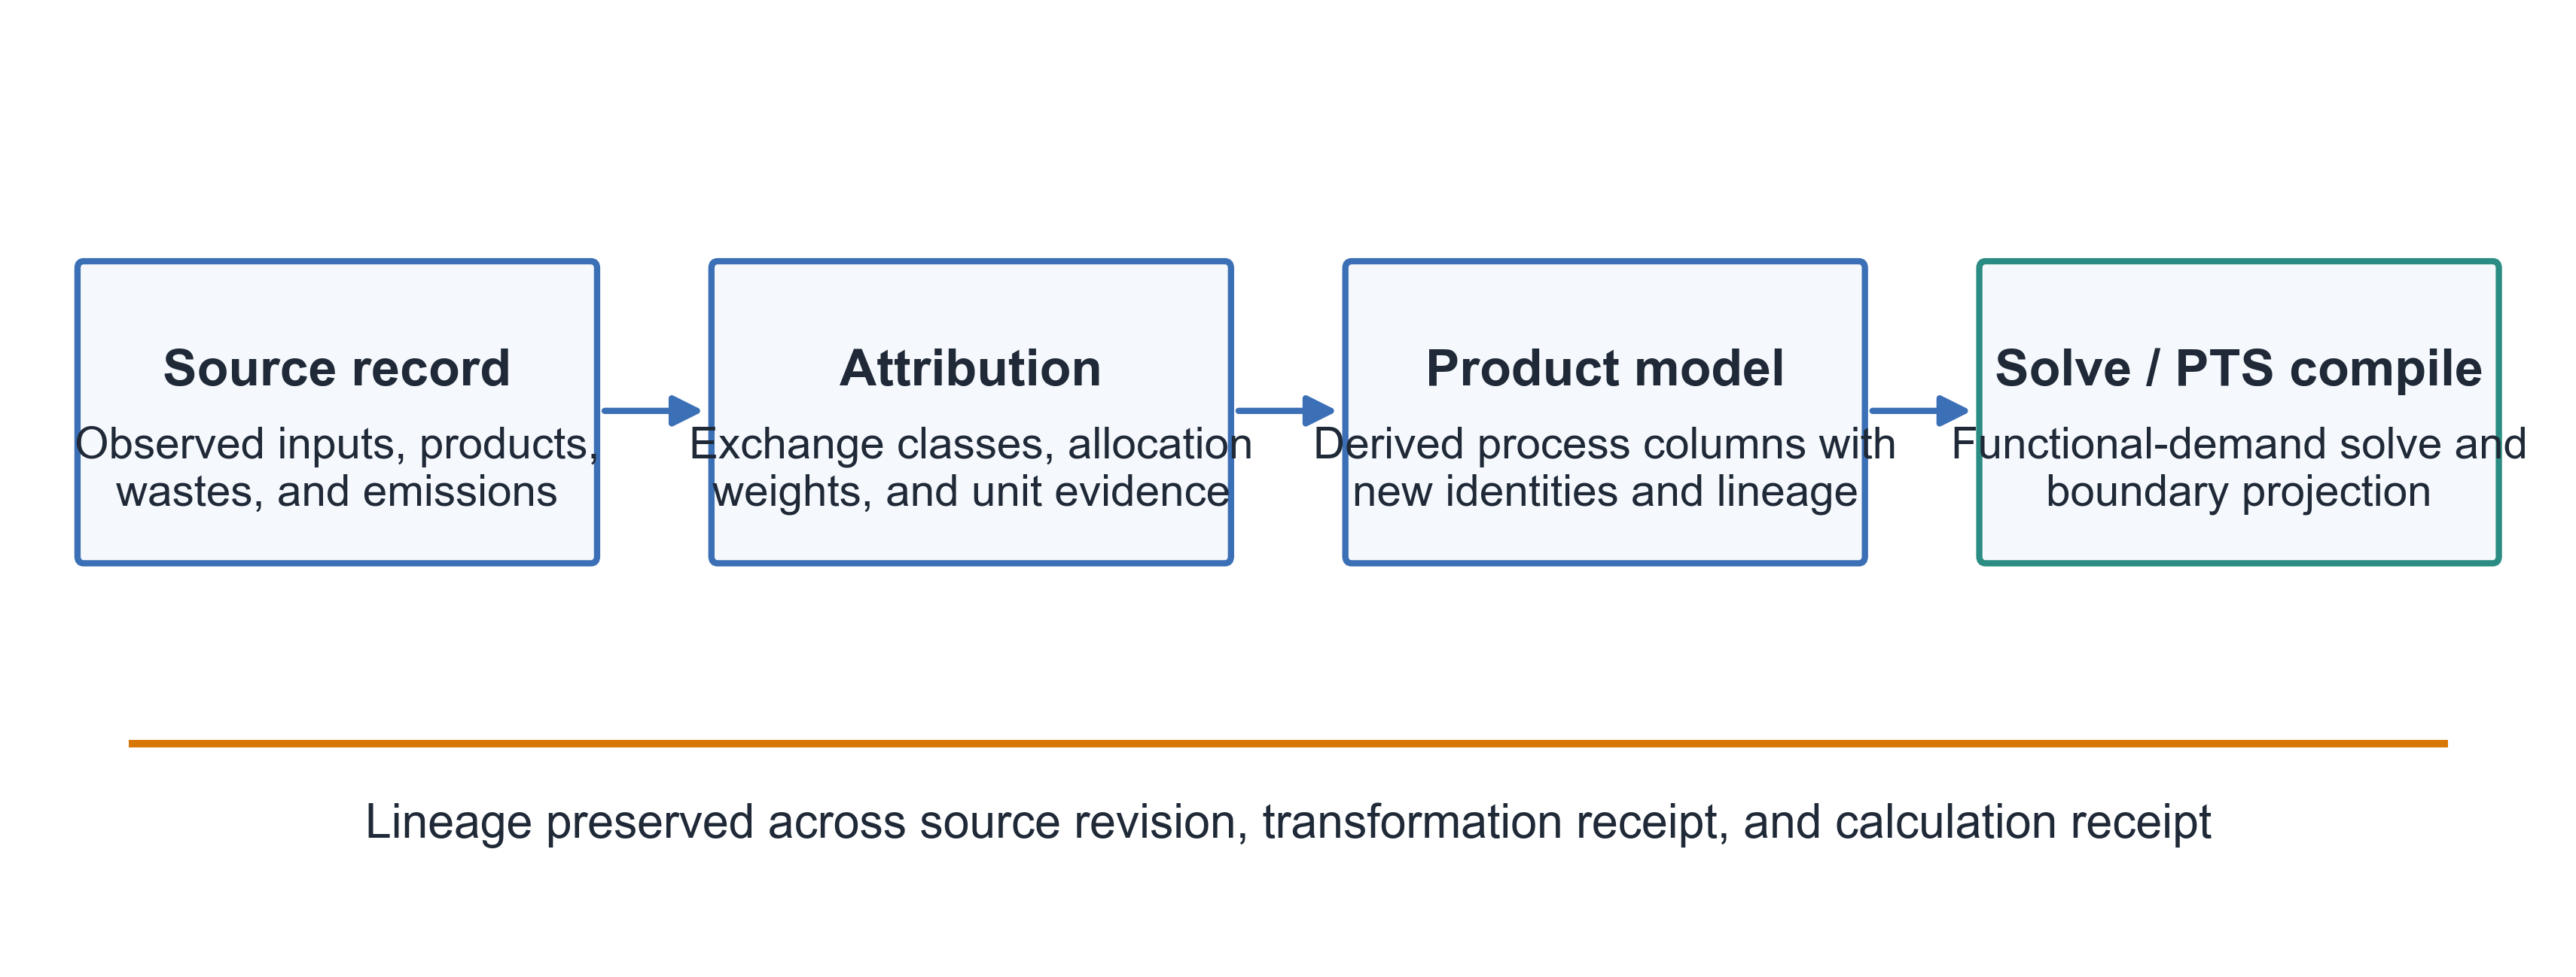
\includegraphics[width=6.5in,height=\textheight,keepaspectratio]{figures/figure1_method_chain.png}

}

\caption{The traceable transformation chain separates the total-process
source record, attribution evidence, product-resolved computation, and
system solution or PTS compilation. The lower line denotes continuous
provenance across the transformations.}

\end{figure}%

\newpage

\begin{figure}[H]

{\centering 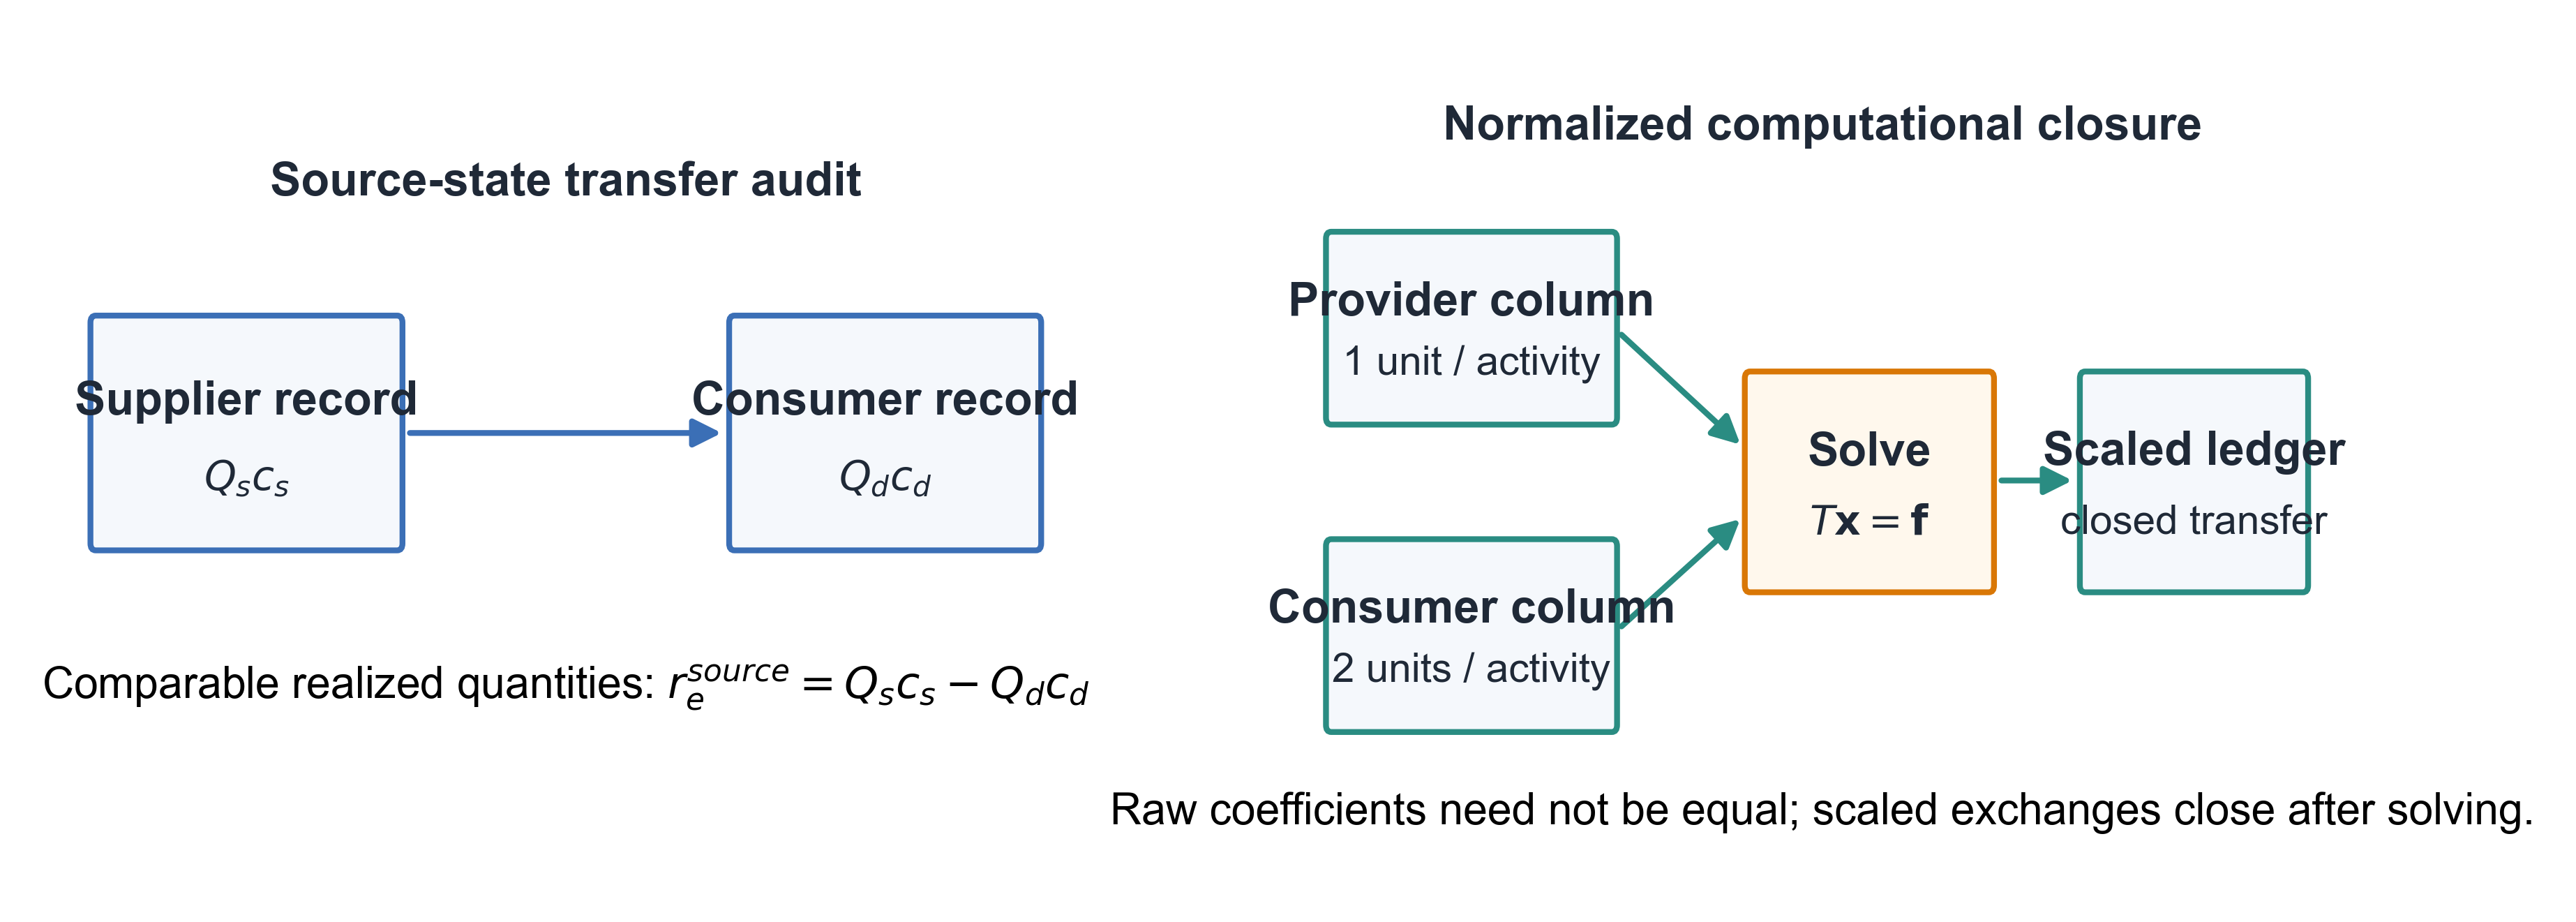
\includegraphics[width=6.5in,height=\textheight,keepaspectratio]{figures/figure2_quantity_semantics.png}

}

\caption{Source-state transfer equality and normalized computational
closure are different properties. The left panel compares realized
quantities on a common source basis. The right panel shows how unequal
raw coefficients close after multiplication by their solved activities.}

\end{figure}%

\subsection{3.5. Lineage model}\label{lineage-model}

The lineage model can be expressed using the generic
entity-activity-agent pattern of W3C PROV {[}20{]}. Source processes,
flows, unit groups, and evidence documents are entities. Attribution and
compilation are activities with declared parameters and software
versions. Product-resolved processes, compiled boundary artifacts,
comparison reports, and figures are derived entities. This mapping is
optional for file format, but the semantic distinctions are mandatory.

The minimum lineage chain is: (i) source revision to product-resolved
revision, documented by an attribution receipt; (ii) product-resolved
revision to scaled exchanges and LCI/LCIA, documented by an immutable
model snapshot and solve receipt; and (iii) scaled results to a PTS
boundary artifact, documented by a compilation receipt.

Every result must be resolvable to an immutable source snapshot and
transformation parameters. ``Latest version'' references are
insufficient for a reproducibility package.

\section{4. Mathematical formulation}\label{mathematical-formulation}

\subsection{4.1. Explicit product
attribution}\label{explicit-product-attribution}

Consider total-process source \(j\) with co-products \(k\in K_j\) and
observed product quantities \(q_{jk}>0\). Let
\(\mathbf{s}_j\in\mathbb{R}^{m}\) be the vector of total exchanges
classified as shared and allocable. Let
\(\mathbf{p}_{jk}\in\mathbb{R}^{m}\) be the total exchanges assigned
specifically to product \(k\) during the same source period.
Reference-product outputs, substitution exchanges, and other
nonpartitioned controls are excluded from these vectors and handled by
their own rules.

Let \(w_{jk}\geq 0\) be the allocation weight for product \(k\),
expressed on a declared common basis. At least one weight must be
positive. The normalized factor is

\[
\alpha_{jk}=\frac{w_{jk}}{\sum_{\ell\in K_j} w_{j\ell}},
\qquad
\sum_{k\in K_j}\alpha_{jk}=1.
\tag{1}
\]

The product-resolved exchange vector per unit of product \(k\) is

\[
\widetilde{\mathbf e}_{jk}
=
\frac{\alpha_{jk}\mathbf{s}_j+\mathbf{p}_{jk}}{q_{jk}}.
\tag{2}
\]

This equation supports quantity, mass, energy, economic, or manual
weights only when their basis and dimensions are explicit. For products
in different unit groups, an evidence-bearing transformation is
required. Density can convert volume to mass; lower heating value can
convert mass to energy; a user-defined factor can be used only if its
dimensions, value, applicability, and source are recorded. A
price-derived factor is called economic allocation only if currency,
price year, geography, market stage, taxes, and zero- or negative-value
rules are fixed.

\textbf{Proposition 1 (allocation closure).} If all shared exchanges are
partitioned by Eq. (1), each product-specific exchange is assigned once,
and the same source-period product quantities are used in Eq. (2), then

\[
\sum_{k\in K_j}q_{jk}\widetilde{\mathbf e}_{jk}
=
\mathbf{s}_j+\sum_{k\in K_j}\mathbf{p}_{jk}.
\tag{3}
\]

\textbf{Proof.} Substituting Eq. (2) into the left-hand side gives
\(\sum_k(\alpha_{jk}\mathbf{s}_j+\mathbf{p}_{jk})\). By Eq. (1),
\(\sum_k\alpha_{jk}=1\), yielding Eq. (3). \(\square\)

Equation (3) is an accounting identity over the classified exchange
vectors. It is not a proof of elemental or total mass balance. The
transformation fails closed when the reference quantity is zero or
missing, weights are incomplete, a required conversion lacks evidence, a
product-specific exchange is assigned more than once, or a declared
allocation set cannot be normalized.

\subsection{4.2. Full product-system
calculation}\label{full-product-system-calculation}

After product resolution, the product system is represented by a signed
technology-system matrix

\[
T\in\mathbb{R}^{n\times n},
\]

where row \(i\) denotes a product or intermediate-flow balance and
column \(j\) denotes a process activity. The sign convention used here
is

\begin{itemize}
\tightlist
\item
  \(T_{ij}>0\) for production of row flow \(i\) by activity \(j\);
\item
  \(T_{ij}<0\) for consumption of row flow \(i\) by activity \(j\); and
\item
  \(f_i>0\) for required net output of row flow \(i\).
\end{itemize}

For a nonsingular square system,

\[
T\mathbf{x}=\mathbf{f},
\qquad
\mathbf{x}=T^{-1}\mathbf{f},
\tag{4}
\]

with \(\mathbf{x},\mathbf{f}\in\mathbb{R}^{n}\). Implementations should
solve the linear system rather than explicitly form \(T^{-1}\).

Let

\[
B\in\mathbb{R}^{m_e\times n}
\]

be the elementary-flow matrix and

\[
C\in\mathbb{R}^{m_i\times m_e}
\]

the characterization matrix. The life cycle inventory and impact vectors
are

\[
\mathbf{z}=B\mathbf{x}\in\mathbb{R}^{m_e},
\tag{5}
\]

\[
\mathbf{h}=C\mathbf{z}=CB\mathbf{x}\in\mathbb{R}^{m_i}.
\tag{6}
\]

The symbols have distinct meanings: \(\mathbf{x}\) is the process
activity vector; scaled exchanges are process coefficients multiplied by
their corresponding activities; \(\mathbf{z}\) is the elementary-flow
inventory; and \(\mathbf{h}\) is the characterized impact result. A
contribution matrix must not be relabeled as an activity vector.

A scale-aware solver residual is

\[
\rho_T=
\frac{\lVert T\widehat{\mathbf{x}}-\mathbf{f}\rVert}
{\lVert T\rVert\lVert\widehat{\mathbf{x}}\rVert+\lVert\mathbf{f}\rVert},
\tag{7}
\]

where \(\widehat{\mathbf{x}}\) is the computed solution. For a declared
intermediate-flow row, the activity-scaled production, consumption, and
final demand must reproduce the corresponding row of
\(T\widehat{\mathbf{x}}-\mathbf f\) within tolerance. An MFA or Sankey
diagram used as evidence must therefore be generated from the scaled
exchange ledger, not from raw normalized coefficients.

\subsection{4.3. Product technology
system}\label{product-technology-system}

A PTS is a declared internal subsystem with \(p\) normalized process
activities and \(r\) exposed product interfaces. Its dependency equation
is

\[
\mathbf{x}_{\mathrm{pts}}
=A_{\mathrm{pts}}\mathbf{x}_{\mathrm{pts}}+D\mathbf{y},
\tag{8}
\]

where

\begin{itemize}
\tightlist
\item
  \(A_{\mathrm{pts}}\in\mathbb{R}^{p\times p}\) contains internal
  activity dependencies after product selection, allocation, and unit
  conversion;
\item
  \(D\in\mathbb{R}^{p\times r}\) maps exposed-product demand
  \(\mathbf y\in\mathbb{R}^{r}\) to the corresponding internal reference
  producers; and
\item
  \(\mathbf{x}_{\mathrm{pts}}\in\mathbb{R}^{p}\) is the internal
  activity vector.
\end{itemize}

Define

\[
M=I-A_{\mathrm{pts}}.
\tag{9}
\]

Compilation requires \(M\) to be nonsingular. A sufficient, but not
necessary, condition for a nonnegative dependency matrix is
\(\rho(A_{\mathrm{pts}})<1\), where \(\rho\) is the spectral radius.
Numerical acceptance also depends on conditioning, not only
nonsingularity.

Let

\[
G_{\mathrm{pts}}\in\mathbb{R}^{m_b\times p}
\]

project internal activities to declared boundary technosphere exchanges,
and let

\[
B_{\mathrm{pts}}\in\mathbb{R}^{m_e\times p}
\]

contain the internal elementary-flow coefficients. Rows of
\(G_{\mathrm{pts}}\) are identified boundary products, wastes, or
intermediate flows. Internal production and consumption of a closed flow
cancel in the net boundary projection; allowed external inputs and
outputs remain visible. Rows of \(B_{\mathrm{pts}}\) use elementary-flow
identities compatible with the chosen characterization matrix.

Instead of solving separately for arbitrary demands, the compiler solves
the multiple-right-hand-side system

\[
MX=D
\tag{10}
\]

for

\[
X=M^{-1}D\in\mathbb{R}^{p\times r}.
\]

The compiled boundary and elementary-flow operators are

\[
\overline G=G_{\mathrm{pts}}X\in\mathbb{R}^{m_b\times r},
\tag{11}
\]

\[
\overline B=B_{\mathrm{pts}}X\in\mathbb{R}^{m_e\times r}.
\tag{12}
\]

Each column corresponds to one exposed-product basis demand. The
compilation receipt records the ordered row and column identities of
\(A_{\mathrm{pts}}\), \(D\), \(G_{\mathrm{pts}}\), and
\(B_{\mathrm{pts}}\); source revisions; product-provider choices; units;
boundary policy; solver version; condition estimate; residuals; and
output hashes.

\newpage

\begin{figure}[H]

{\centering 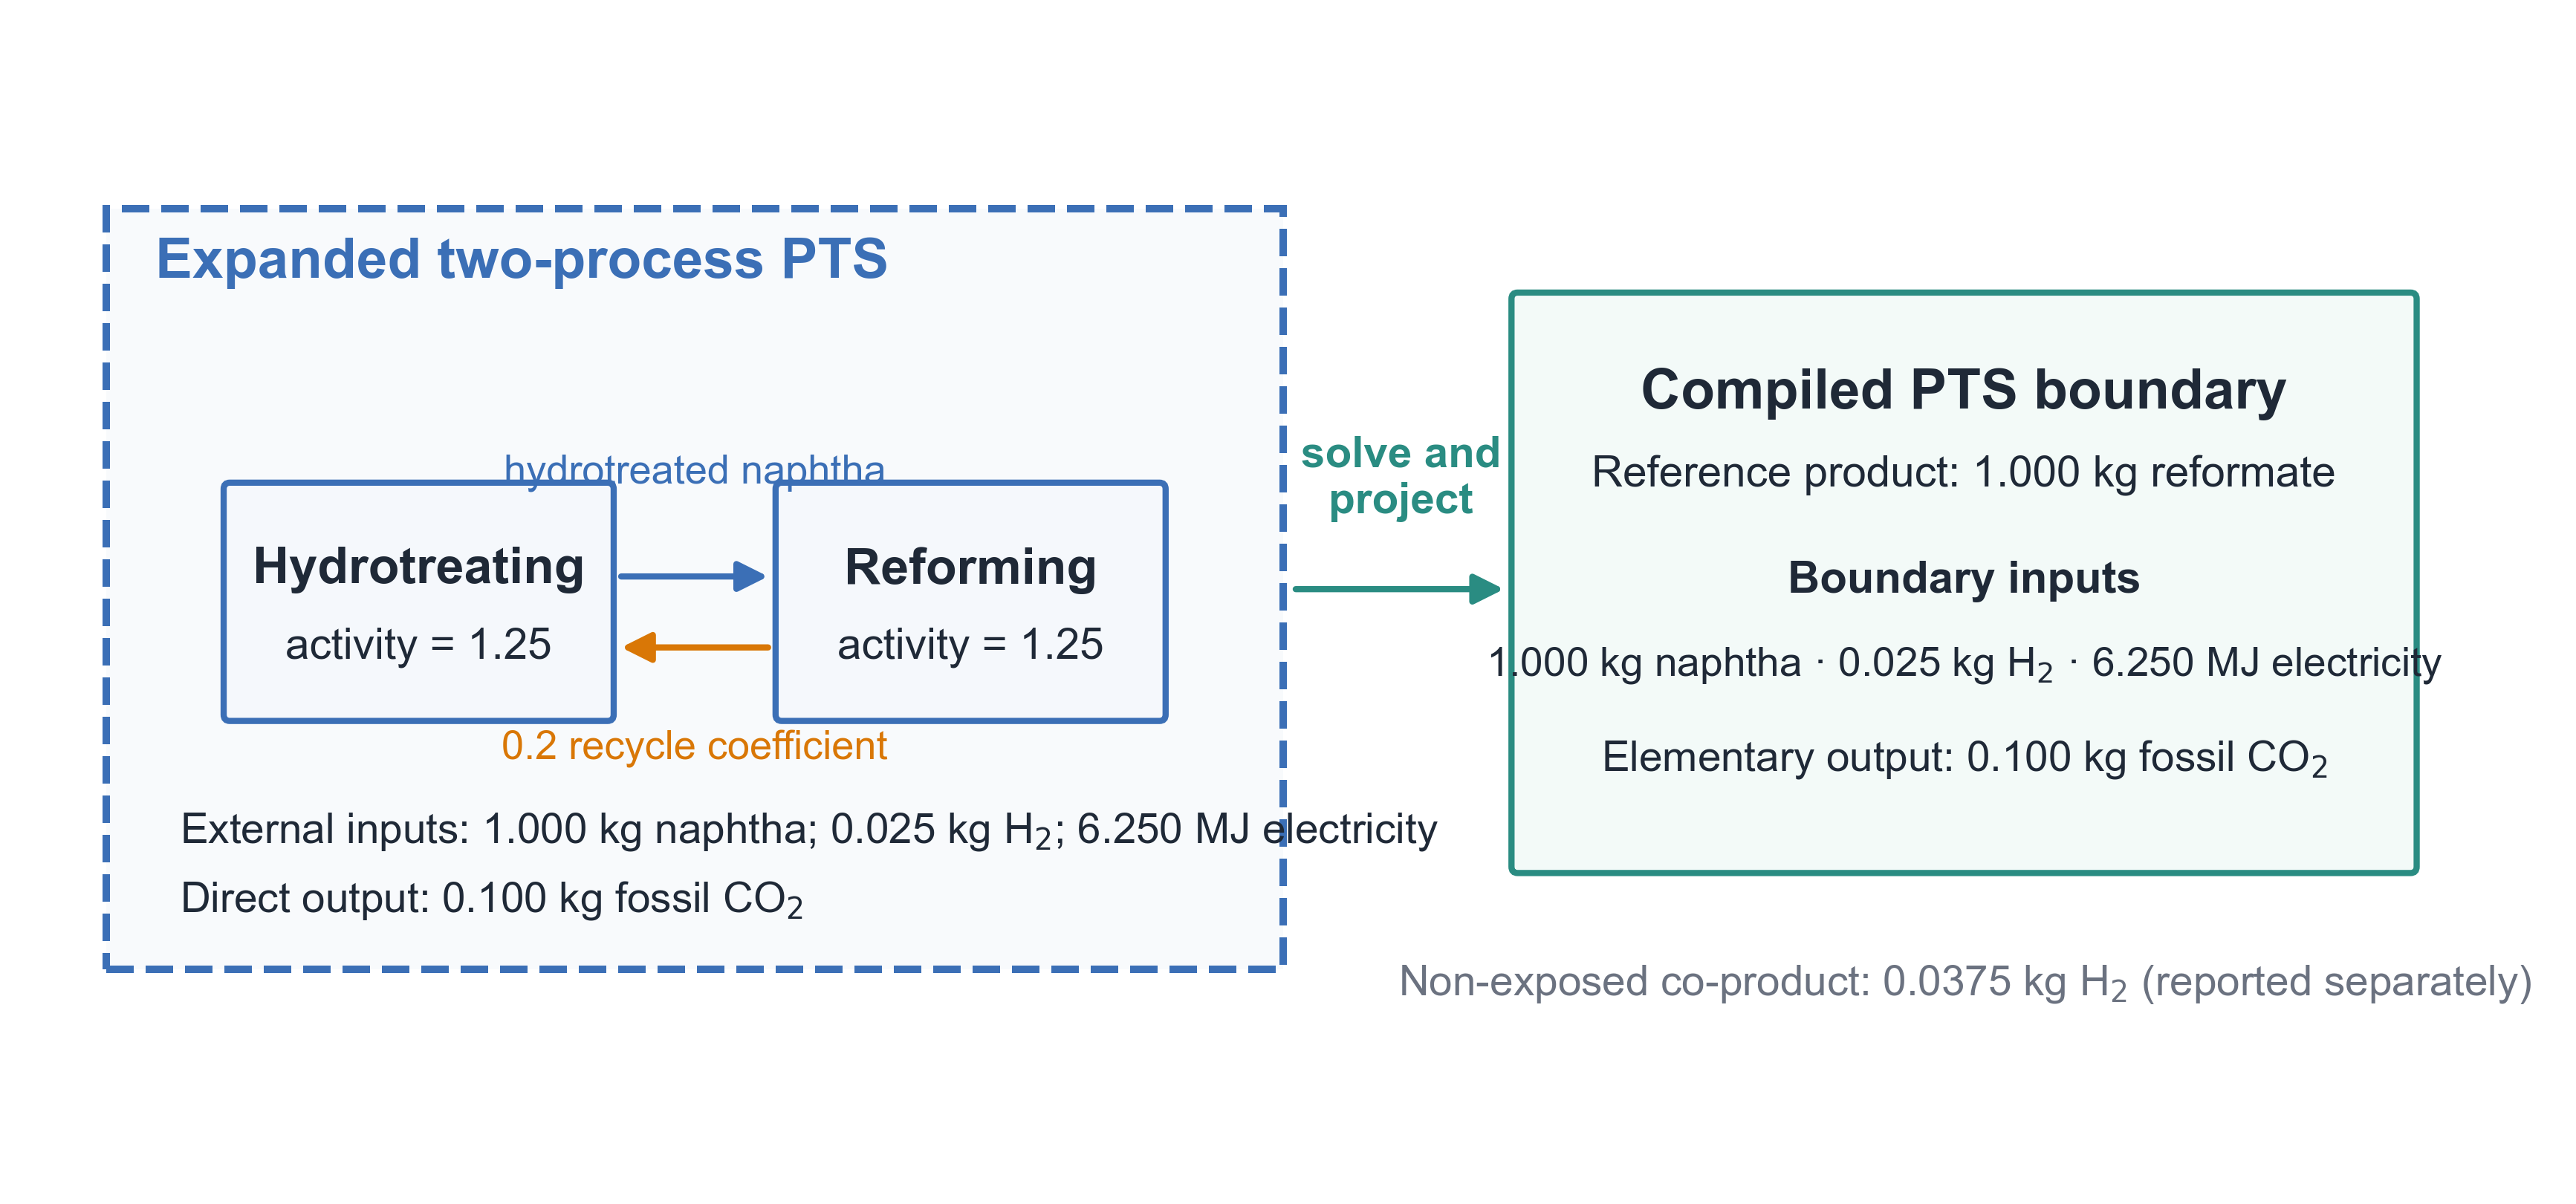
\includegraphics[width=6.5in,height=\textheight,keepaspectratio]{figures/figure3_pts_operator.png}

}

\caption{Case 5 PTS compilation. The expanded hydrotreating-reforming
subsystem is solved for one kilogram of reformate and projected onto the
declared interface. The four exposed nonzero components are preserved
exactly; the non-exposed hydrogen co-product is reported separately.}

\end{figure}%

\subsection{4.4. Boundary-operator
equivalence}\label{boundary-operator-equivalence}

\textbf{Proposition 2 (PTS boundary-operator equivalence).} Assume that:

\begin{enumerate}
\def\labelenumi{\arabic{enumi}.}
\tightlist
\item
  \(M=I-A_{\mathrm{pts}}\) is nonsingular;
\item
  coefficients, allocation factors, provider mappings, units, and
  boundary classifications are fixed over the declared demand domain;
\item
  \(D\) maps each exposed product to a unique, declared internal
  reference producer or a uniquely defined linear combination; and
\item
  the expanded subsystem and compiled artifact use the same row
  identities, sign convention, and boundary definition.
\end{enumerate}

Then, for every exposed-product demand \(\mathbf y\) in the declared
linear demand domain, the expanded subsystem and compiled artifact
return identical boundary technosphere, elementary-flow, and
characterized impact vectors in exact arithmetic:

\[
\mathbf g_{\mathrm{expanded}}(\mathbf y)
=
\overline G\mathbf y,
\tag{13}
\]

\[
\mathbf b_{\mathrm{expanded}}(\mathbf y)
=
\overline B\mathbf y,
\tag{14}
\]

\[
\mathbf h_{\mathrm{expanded}}(\mathbf y)
=
C\overline B\mathbf y.
\tag{15}
\]

\textbf{Proof.} From Eqs. (8)-(10), the expanded internal solution is
\(\mathbf{x}_{\mathrm{pts}}=M^{-1}D\mathbf y=X\mathbf y\). Boundary
projection gives
\(\mathbf g=G_{\mathrm{pts}}X\mathbf y=\overline G\mathbf y\), and
elementary-flow projection gives
\(\mathbf b=B_{\mathrm{pts}}X\mathbf y=\overline B\mathbf y\). Applying
the same characterization matrix yields Eq. (15). \(\square\)

This proposition is a statement about the declared linear model, not
proof that a particular implementation built the matrices correctly.
Software conformance requires an independent oracle. Because both
representations are linear maps from \(\mathbb{R}^r\), equality of their
operator columns - equivalently, equality for the \(r\) canonical basis
demands - is sufficient to establish equality over the full linear
demand space. Testing one demand establishes only a single point.
Testing several nonspanning demands provides stronger empirical evidence
but does not by itself establish operator equality.

The evidence levels used in this paper are therefore:

\begin{itemize}
\tightlist
\item
  \textbf{Level A - single-point agreement:} one product and one demand
  vector;
\item
  \textbf{Level B - multi-demand agreement:} several products or demand
  vectors, without a basis-complete operator oracle; and
\item
  \textbf{Level C - boundary-operator equivalence:} direct comparison of
  \(\overline G\) and \(\overline B\), or basis-complete comparison
  against an independently constructed expanded oracle, together with
  the assumptions of Proposition 2.
\end{itemize}

``Semantics-preserving compilation'' is reserved for a validated Level C
implementation within the declared boundary and demand domain. Levels A
and B support only ``numerically equivalent for the tested cases.''

\newpage

\subsection{4.5. Numerical contract}\label{numerical-contract}

A small solve residual does not guarantee an accurate solution when
\(M\) is ill-conditioned. Each compiled artifact therefore reports:

\begin{itemize}
\tightlist
\item
  dimensions and nonzero counts of \(A_{\mathrm{pts}}\), \(M\), \(D\),
  \(G_{\mathrm{pts}}\), and \(B_{\mathrm{pts}}\);
\item
  a condition-number estimate \(\kappa(M)\) in a declared norm;
\item
  multiple-right-hand-side solve residuals;
\item
  component-wise differences between independent expanded and compiled
  oracles;
\item
  the product-interface normalization residual; and
\item
  an error budget tied to the case tolerances.
\end{itemize}

For computed \(\widehat X\), the scale-aware PTS residual is

\[
\rho_M=
\frac{\lVert M\widehat X-D\rVert}
{\lVert M\rVert\lVert\widehat X\rVert+\lVert D\rVert}.
\tag{16}
\]

Conditioning is interpreted relative to machine precision \(u\) and the
required result accuracy. A case manifest defines a numerical error
budget \(\tau_{\mathrm{num}}\) and rejects compilation when the
estimated amplification \(\kappa(M)u\) is inconsistent with that budget.
This is preferable to one universal condition-number threshold. The
implementation solves \(MX=D\) using a documented linear solver and must
not use a numerically unnecessary explicit inverse {[}23{]}.

\subsection{4.6. Fail-closed conditions}\label{fail-closed-conditions}

Compilation or product resolution is rejected when any of the following
applies:

\begin{itemize}
\tightlist
\item
  missing or zero product reference quantity;
\item
  incomplete, nonfinite, or nonnormalizable attribution weights;
\item
  cross-unit or cross-property conversion without evidence;
\item
  identity or version conflict for a linked flow;
\item
  incompatible flow property or unit group;
\item
  unresolved multiple providers for a required internal product;
\item
  nonunique or missing exposed-product producer;
\item
  undeclared boundary port or row identity;
\item
  singular or insufficiently stable internal system under the case error
  budget;
\item
  stale artifact whose source, boundary, allocation, or compiler hash no
  longer matches;
\item
  unsupported nested PTS structure; or
\item
  an exchange class whose required treatment is not defined.
\end{itemize}

A rejected negative case is a successful validation outcome when
rejection is the predeclared oracle. Silent fallback to names,
``latest'' versions, default ratios, or provider ordering is not
permitted.

\section{5. Interoperability and provenance
contract}\label{interoperability-and-provenance-contract}

The interoperability claim is intentionally field-level. A package can
be syntactically valid while losing a field, normalizing a quantity, or
moving information into an extension. A complete ILCD/TIDAS round-trip
evaluation must therefore classify each relevant field as
\emph{preserved}, \emph{normalized}, \emph{extension-dependent},
\emph{unsupported}, or \emph{rejected}. The five benchmarks reported
below exercise versioned graph snapshots and flow identities, but they
do not constitute that complete round-trip evaluation.

\textbf{Table 3. Standard-to-computation semantic crosswalk.}

{\def\LTcaptype{none} % do not increment counter
\begin{longtable}[]{@{}
  >{\raggedright\arraybackslash}p{(\linewidth - 4\tabcolsep) * \real{0.3333}}
  >{\raggedright\arraybackslash}p{(\linewidth - 4\tabcolsep) * \real{0.3333}}
  >{\raggedright\arraybackslash}p{(\linewidth - 4\tabcolsep) * \real{0.3333}}@{}}
\toprule\noalign{}
\begin{minipage}[b]{\linewidth}\raggedright
Object or field
\end{minipage} & \begin{minipage}[b]{\linewidth}\raggedright
Identity and computational treatment
\end{minipage} & \begin{minipage}[b]{\linewidth}\raggedright
Required validation
\end{minipage} \\
\midrule\noalign{}
\endhead
\bottomrule\noalign{}
\endlastfoot
Flow UUID and version & Retain for supported source flows; use as
matrix-row and exchange identity; map only through an explicit receipt.
& Import-export-reimport equality, version-conflict rejection, and
name-collision negative case. \\
Flow property, unit group, and unit & Retain or explicitly normalize;
use the property as the quantity basis and record every conversion. &
Round trip, compatible-unit invariance, incompatible-unit rejection, and
conversion-evidence check. \\
Source process UUID and version & Retain as the source-fact identity;
never reuse for product-resolved or compiled objects. & Round trip,
identity separation, and stale-source detection. \\
Product quantities and attribution metadata & Retain reporting basis;
use as the attribution denominator and reference output; preserve the
rule in native fields or a provenance receipt. & Allocation closure,
zero-quantity rejection, rule completeness, and re-import
reproducibility. \\
Product-resolved process & Create a new identity; use as a normalized
computational column; link to the source process and receipt. &
Derived-identity check and reconstitution of the same product
inventory. \\
PTS boundary artifact & Create a new identity; use as a reusable
compiled column set; bind source, boundary, matrix, and solver receipts.
& Expanded-compiled operator oracle, condition and residual report, and
stale-artifact rejection. \\
Multilingual names and classifications & Preserve as descriptive fields
where supported; do not substitute them for identity. & Field-level
round trip and deliberate duplicate-name case. \\
\end{longtable}
}

ILCD UUID/version guidance supports the source-identity part of this
contract {[}4{]}. TIDAS provides the versioned schema surface to be
pinned for the test package {[}5{]}. Neither standard is presumed to
encode every compiler-specific receipt field. When the target profile
lacks a native field, provenance can be carried in a declared extension
or companion receipt; it must not be silently discarded.

\section{6. Progressive benchmark
design}\label{progressive-benchmark-design}

\subsection{6.1. Benchmark scope and
execution}\label{benchmark-scope-and-execution}

The implementation was evaluated through five projects that form one
progressively composed refinery-inspired benchmark family. Each project
was created through the public application programming interface, and
each project after the first was duplicated from its predecessor before
adding the next modeling feature. This preserves a visible derivation
chain while keeping each stage independently executable. All material
and emission quantities are declared benchmark assumptions. They are
intended to expose allocation, connection, normalized-supply,
recycle-loop, system-solution, and PTS-compilation behavior; they are
not measured refinery data and are not intended to represent average or
best-available refinery performance.

The functional demands progress from 1 kg straight-run naphtha in Case 1
to 1 kg finished gasoline in Cases 2-5. Case 2 establishes a balanced
four-process foreground. Case 3 adds one normalized electricity-supply
process serving multiple units. Case 4 adds a recycle connection between
reforming and hydrotreating. Case 5 compiles the cyclic upgrading
subsystem as a PTS. The same exact elementary-flow identity for fossil
carbon dioxide is used across the cases, and the reported impact vector
is calculated with the implementation's EF 3.1 method set. Because the
benchmark contains only a narrow elementary-flow inventory, the LCIA
vector is used as a propagation and equivalence check, not as a
comparative environmental assessment of refinery technologies.

\begin{figure}[H]

{\centering 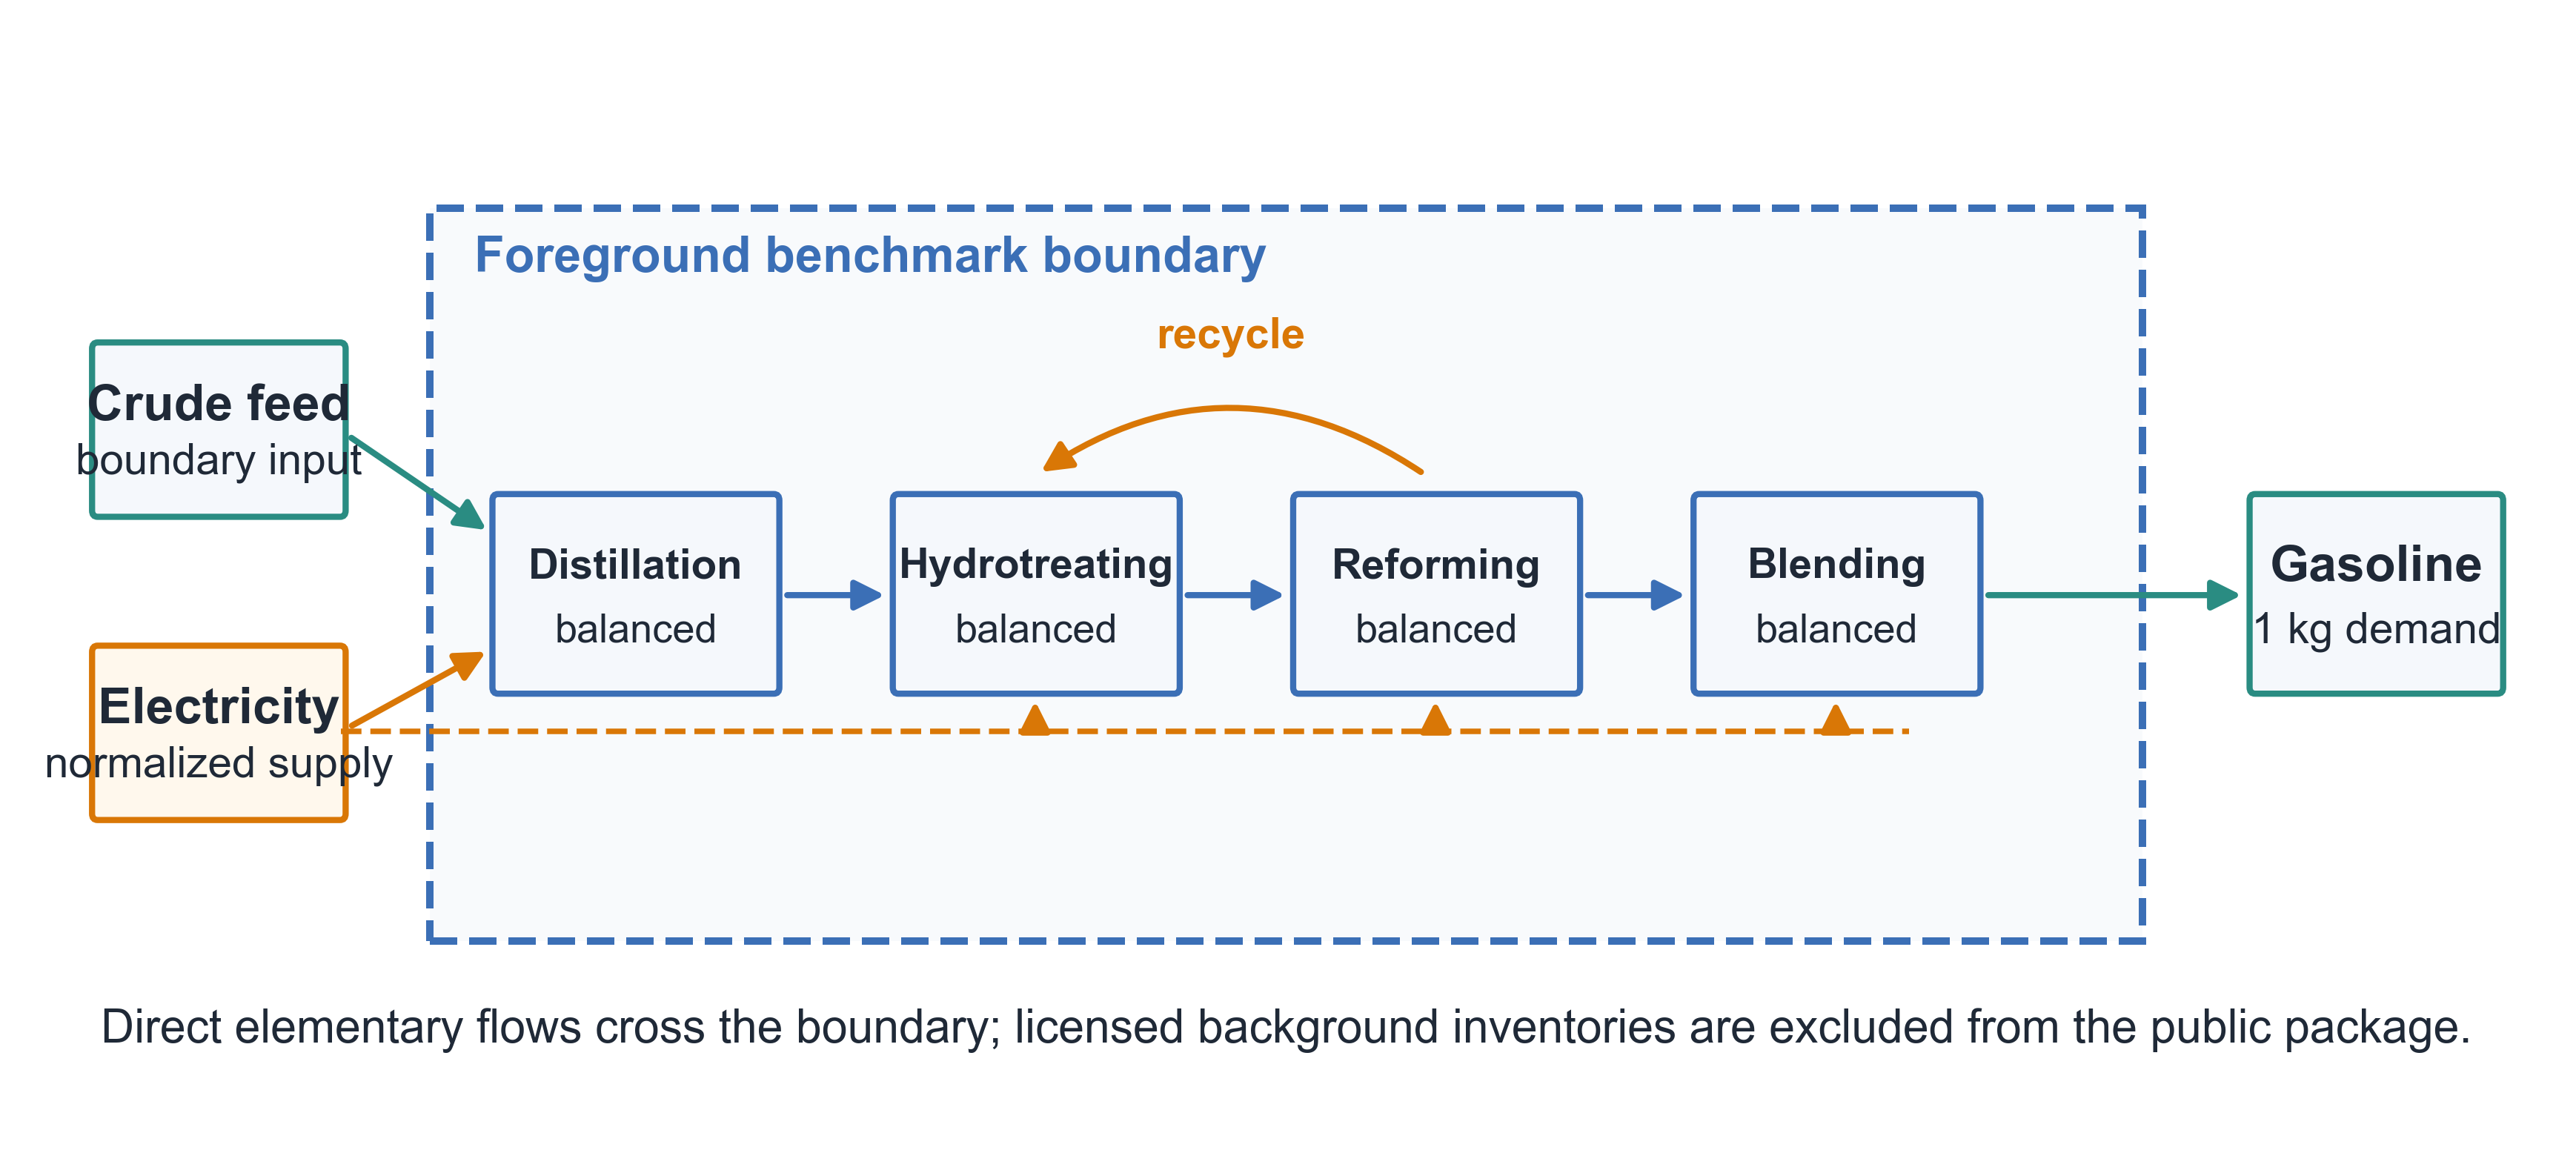
\includegraphics[width=6.5in,height=\textheight,keepaspectratio]{figures/figure4_system_boundary.pdf}

}

\caption{System boundary of the public refinery-inspired benchmark. Four
balanced foreground processes, a normalized electricity supplier, and
the reforming-to-hydrotreating recycle connection are shown. Direct
elementary flows cross the foreground boundary, whereas licensed
background inventories are not redistributed.}

\end{figure}%

Each executed package contains:

\begin{enumerate}
\def\labelenumi{\arabic{enumi}.}
\tightlist
\item
  an immutable input snapshot and schema version;
\item
  flow, process, unit, and boundary index maps;
\item
  allocation and conversion evidence;
\item
  expected positive outcomes and audit conditions;
\item
  graph and result identities needed to distinguish consumer and
  provider representations;
\item
  raw solver and compiler outputs;
\item
  connection residuals and, where available, component-wise comparisons;
\item
  provenance and transformation receipts;
\item
  plotting data and figures;
\item
  software and environment information; and
\item
  a SHA-256 manifest covering all package files.
\end{enumerate}

For a scalar or vector component with reference value
\(y_{\mathrm{ref}}\), a calculation passes when

\[
|y_{\mathrm{calc}}-y_{\mathrm{ref}}|
\leq
\varepsilon_{\mathrm{abs}}
+
\varepsilon_{\mathrm{rel}}|y_{\mathrm{ref}}|.
\tag{17}
\]

Near-zero quantities are interpreted primarily through absolute error.
For nonzero quantities, absolute and relative errors are both reported.
The PTS comparison used an absolute tolerance of \(10^{-10}\) fixed by
the benchmark audit. No tolerance was selected after seeing the result.

\subsection{6.2. Five progressive cases}\label{five-progressive-cases}

\textbf{Table 4. Executed benchmark cases and evidence scope.}

{\def\LTcaptype{none} % do not increment counter
\begin{longtable}[]{@{}
  >{\raggedright\arraybackslash}p{(\linewidth - 6\tabcolsep) * \real{0.2500}}
  >{\raggedright\arraybackslash}p{(\linewidth - 6\tabcolsep) * \real{0.2500}}
  >{\raggedright\arraybackslash}p{(\linewidth - 6\tabcolsep) * \real{0.2500}}
  >{\raggedright\arraybackslash}p{(\linewidth - 6\tabcolsep) * \real{0.2500}}@{}}
\toprule\noalign{}
\begin{minipage}[b]{\linewidth}\raggedright
Case
\end{minipage} & \begin{minipage}[b]{\linewidth}\raggedright
Composition and functional demand
\end{minipage} & \begin{minipage}[b]{\linewidth}\raggedright
Principal audit
\end{minipage} & \begin{minipage}[b]{\linewidth}\raggedright
Evidence level and boundary
\end{minipage} \\
\midrule\noalign{}
\endhead
\bottomrule\noalign{}
\endlastfoot
1. Multi-output unit process & Atmospheric distillation; 1 kg
straight-run naphtha & Allocation closure for every classified shared
exchange and a duplicated-assignment negative control & The source
vector was reconstructed with
\(\lVert\Delta\mathbf e\rVert_\infty=1.39\times10^{-17}\); the negative
control was rejected. \\
2. Balanced foreground chain & Distillation, hydrotreating, reforming,
and blending; 1 kg finished gasoline & Four solved activities and three
activity-scaled connection residuals & All declared internal residuals
were zero. \\
3. Mixed balanced-normalized system & Case 2 plus one normalized
electricity supplier serving four processes & Aggregated normalized
supply and seven connection residuals & Electricity activity was 6.1 MJ;
every declared residual was zero. \\
4. Recycle-loop system & Case 3 plus reforming-to-hydrotreating recycle
& Open-loop versus recycle-loop activity and boundary comparison & The
recycle changed hydrotreating and reforming activities from 0.8 to 1.0
and changed the boundary ledger. \\
5. PTS-integrated system & Case 4 with hydrotreating and reforming
compiled as a PTS & Independent reconstruction of \(A_{\mathrm{pts}}\),
\(M\), declared boundary inputs, elementary flows, and the tested LCIA
vector & \(\kappa_1(M)=5.0\), \(\rho_M=0\), and all four nonzero
declared components agreed exactly. \\
\end{longtable}
}

\subsubsection{Case 1: multi-output atmospheric
distillation}\label{case-1-multi-output-atmospheric-distillation}

The first project contains one atmospheric-distillation process with
straight-run naphtha, diesel cut, and residue represented as multiple
outputs. Their quantity-based factors are 0.25, 0.45, and 0.30. An
independent script applied Eq. (2) to every classified shared exchange,
multiplied each product-resolved coefficient by its product quantity,
and reconstructed the source vector. The absolute residuals were zero to
floating-point precision:
\(\lVert\Delta\mathbf e\rVert_\infty=1.39\times10^{-17}\) and
\(\lVert\Delta\mathbf e\rVert_2=1.39\times10^{-17}\). A negative control
assigned a 0.4-unit product-specific exchange to two product columns,
produced a 0.4-unit residual, and was rejected.

\subsubsection{Case 2: balanced four-process
foreground}\label{case-2-balanced-four-process-foreground}

The second project extends the source process into a four-process
balanced foreground. For 1 kg finished gasoline, the activities were
0.84 for distillation, 0.8 for hydrotreating, 0.8 for reforming, and 1.0
for blending. The naphtha, hydrotreated-naphtha, and reformate transfers
each had an activity-scaled absolute residual of 0.0 kg. The aggregate
fossil-carbon-dioxide inventory was 0.09 kg.

\subsubsection{Case 3: normalized electricity supply combined with
balanced
processes}\label{case-3-normalized-electricity-supply-combined-with-balanced-processes}

The third project keeps the four foreground unit processes in balanced
mode and introduces a normalized electricity supplier. The supplier
serves four consumers without asserting a realized source-state quantity
for each raw coefficient. The solver aggregated 1.6, 2.4, 1.6, and 0.5
MJ of unit-process electricity requirements into a 6.1 MJ supplier
activity. All four electricity links and all three material links had
zero activity-scaled residual. This case isolates the distinction
between normalized computational closure and source-state transfer
auditing.

\subsubsection{Case 4: recycle-loop
comparison}\label{case-4-recycle-loop-comparison}

The fourth project adds a 0.2 kg recycle-naphtha output from reforming
to the corresponding hydrotreating input. Relative to the open-loop
model, hydrotreating and reforming activities increased from 0.8 to 1.0,
distillation decreased from 0.84 to 0.8, and normalized electricity
supply increased from 6.1 to 7.02381 MJ. The fossil-carbon-dioxide
boundary total increased from 0.1144 to 0.133333 kg in this hypothetical
parameterization. These are model-response differences caused by the
declared loop coefficients, not estimates of an industrial recycle
benefit or penalty.

\subsubsection{Case 5: PTS compilation and independent component
oracle}\label{case-5-pts-compilation-and-independent-component-oracle}

The fifth project compiles the cyclic hydrotreating-reforming subsystem.
In node order (hydrotreating, reforming), the independent oracle
reconstructed

\[
A_{\mathrm{pts}}=
\begin{bmatrix}0&1\\0.2&0\end{bmatrix},
\qquad
M=I-A_{\mathrm{pts}}=
\begin{bmatrix}1&-1\\-0.2&1\end{bmatrix}.
\]

For one kilogram of exposed reformate, the internal activity vector was
\((1.25,1.25)^\mathsf{T}\), \(\kappa_1(M)=\kappa_\infty(M)=5.0\), and
the infinity-norm solve residual was zero. The independent projection
and compiled artifact agreed exactly for the three declared nonzero
boundary inputs (1.0 kg naphtha, 0.025 kg make-up hydrogen, and 6.25 MJ
electricity) and the 0.1 kg fossil-carbon-dioxide elementary flow. A
0.0375 kg reformer hydrogen by-product was identified by the oracle but
is not an exposed PTS shell output; it is therefore reported as a
non-exposed row rather than silently treated as a compiled boundary
exchange. The expanded and PTS-integrated models also returned identical
reported EF 3.1 vectors for the tested demand.

\textbf{Table 5. Independent comparison of the tested PTS reformate
column.}

{\def\LTcaptype{none} % do not increment counter
\begin{longtable}[]{@{}
  >{\raggedright\arraybackslash}p{(\linewidth - 10\tabcolsep) * \real{0.1429}}
  >{\raggedright\arraybackslash}p{(\linewidth - 10\tabcolsep) * \real{0.1429}}
  >{\raggedright\arraybackslash}p{(\linewidth - 10\tabcolsep) * \real{0.1429}}
  >{\raggedleft\arraybackslash}p{(\linewidth - 10\tabcolsep) * \real{0.1905}}
  >{\raggedleft\arraybackslash}p{(\linewidth - 10\tabcolsep) * \real{0.1905}}
  >{\raggedleft\arraybackslash}p{(\linewidth - 10\tabcolsep) * \real{0.1905}}@{}}
\toprule\noalign{}
\begin{minipage}[b]{\linewidth}\raggedright
Exchange
\end{minipage} & \begin{minipage}[b]{\linewidth}\raggedright
Role
\end{minipage} & \begin{minipage}[b]{\linewidth}\raggedright
Unit and direction
\end{minipage} & \begin{minipage}[b]{\linewidth}\raggedleft
Independent calculation
\end{minipage} & \begin{minipage}[b]{\linewidth}\raggedleft
Compiled PTS
\end{minipage} & \begin{minipage}[b]{\linewidth}\raggedleft
Absolute difference
\end{minipage} \\
\midrule\noalign{}
\endhead
\bottomrule\noalign{}
\endlastfoot
Straight-run naphtha & Boundary input & kg, input & 1.000 & 1.000 &
0.000 \\
Make-up hydrogen & Boundary input & kg, input & 0.025 & 0.025 & 0.000 \\
Refinery electricity supply & Boundary input & MJ, input & 6.250 & 6.250
& 0.000 \\
Carbon dioxide, fossil & Elementary output & kg, output & 0.100 & 0.100
& 0.000 \\
\end{longtable}
}

The independent calculation additionally identified 0.0375 kg of
reformer by-product hydrogen. Because this co-product is not exposed by
the PTS shell, it is reported separately rather than counted as an
agreement row.

\subsection{6.3. Cross-case validation
matrix}\label{cross-case-validation-matrix}

The five projects are cases in a compositional sequence, whereas the
scientific checks cut across that sequence. Table 6 prevents the number
of projects from being confused with the number of validation
dimensions.

\textbf{Table 6. Cross-case validation status.}

{\def\LTcaptype{none} % do not increment counter
\begin{longtable}[]{@{}
  >{\raggedright\arraybackslash}p{(\linewidth - 4\tabcolsep) * \real{0.3333}}
  >{\raggedright\arraybackslash}p{(\linewidth - 4\tabcolsep) * \real{0.3333}}
  >{\raggedright\arraybackslash}p{(\linewidth - 4\tabcolsep) * \real{0.3333}}@{}}
\toprule\noalign{}
\begin{minipage}[b]{\linewidth}\raggedright
Validation dimension
\end{minipage} & \begin{minipage}[b]{\linewidth}\raggedright
Evidence in this version
\end{minipage} & \begin{minipage}[b]{\linewidth}\raggedright
Remaining work
\end{minipage} \\
\midrule\noalign{}
\endhead
\bottomrule\noalign{}
\endlastfoot
Multi-output representation & Case 1 reconstructs every classified
shared source exchange;
\(\lVert\Delta\mathbf e\rVert_\infty=1.39\times10^{-17}\). & Add
cross-unit allocation cases with independently sourced conversion
evidence. \\
Activity-scaled connection semantics & Cases 2-4 report zero residuals
for all declared internal connections. & Add incompatible-unit and
missing-conversion negative cases. \\
Progressive composition & Cases 1-5 add balanced processes, normalized
supply, a recycle loop, and PTS compilation through project duplication.
& Evaluate larger and measured systems without changing the declared
benchmark status. \\
PTS compilation & Case 5 compiles and publishes an invertible
two-process PTS; the independent oracle reports \(\kappa_1(M)=5.0\) and
\(\rho_M=0\). & Add stale-artifact, singular-matrix, and
multi-output-basis negative cases. \\
Expanded-compiled comparison & Four nonzero declared boundary/elementary
components and all reported EF 3.1 outputs agree for the tested
reformate/gasoline path. & Compare every exposed-product basis column
and define policy for non-exposed co-products. \\
Interoperability & Exact flow identities, versions, graph snapshots, and
separate consumer/provider graph hashes are retained in the case
evidence. & Execute complete ILCD/TIDAS import-export-reimport field
audits. \\
Limited disclosure & The main graph exposes three nodes instead of four
while the PTS retains two internal nodes in its own canvas. & Define
disclosed fields, a threat model, target secrets, and a reconstruction
baseline before making any privacy claim. \\
\end{longtable}
}

The benchmark calculation follows the causal chain

\[
\text{process parameter}
\rightarrow
\text{scaled intermediate flows and direct emissions}
\rightarrow
\text{background demand}
\rightarrow
\text{LCI}
\rightarrow
\text{LCIA}.
\]

The MFA Sankey for Cases 1-4 is generated from the actual
scaled-exchange table returned by each solved project. Decorative or
manually reconciled Sankey values are not treated as numerical evidence.

\subsection{6.4. Evidence packaging and
checking}\label{evidence-packaging-and-checking}

The executed package contains immutable graph snapshots, result
payloads, audits, provenance records, chart data, figures, and a SHA-256
manifest. A separate NumPy script reads the frozen Case 1 and Case 5
graphs and reconstructs allocation closure, the PTS matrices, the tested
activity vector, and identity-indexed boundary and elementary-flow
components without importing the production PTS compiler. This
independent oracle addresses the small-case matrix-construction risk
while remaining limited to the declared benchmark. External reproduction
in a second LCA implementation remains future work.

The result package distinguishes:

\begin{itemize}
\tightlist
\item
  \textbf{semantic validation:} identities, units, classes, and boundary
  meanings;
\item
  \textbf{algebraic validation:} allocation closure and operator
  construction;
\item
  \textbf{numerical validation:} residuals, conditioning, and component
  errors;
\item
  \textbf{round-trip validation:} supported source fields and derived
  lineage after re-import; and
\item
  \textbf{application validation:} progressive composition in a
  refinery-inspired hypothetical foreground.
\end{itemize}

\section{7. Results and claim
boundaries}\label{results-and-claim-boundaries}

\subsection{7.1. Progressive solve
behavior}\label{progressive-solve-behavior}

All five API-executed benchmark audits passed their declared checks.
Cases 1-4 returned activity vectors with the declared
\(T\mathbf x=\mathbf f\) semantics, finite scaled exchanges, inventory
totals, provenance, and EF 3.1 outputs. The independent Case 1 audit
then reconstructed the classified source exchanges from the three
product-resolved columns. Case 3 showed that four normalized electricity
demands are aggregated through a 6.1 MJ supplier activity rather than by
forcing equality among raw coefficients. Case 4 showed that adding the
recycle loop changes both the internal activity vector and the boundary
ledger.

The internal connection audits provide the clearest implementation
evidence for the quantity semantics introduced in Section 3.4. Every
declared connection in Cases 2-4 had zero residual after activity
scaling. These results demonstrate connection-level accounting closure
for the declared benchmark flows. They do not establish elemental mass
balance, energy balance, or stoichiometric validity of the hypothetical
coefficients.

\subsection{7.2. Inventory propagation}\label{inventory-propagation}

The fossil-carbon-dioxide totals were 0.08 kg for the Case 1 naphtha
demand, 0.09 kg for the balanced Case 2 gasoline chain, 0.1144 kg after
adding the normalized electricity supplier in Case 3, and 0.133333 kg
after adding the recycle loop in Case 4. These changes arise solely from
the declared benchmark coefficients and solved activities. They are
deterministic propagation results, not estimates of refinery
greenhouse-gas intensity. The sparse elementary-flow design also means
that the EF 3.1 vector is not a complete environmental profile.

\subsection{7.3. PTS compilation result}\label{pts-compilation-result}

The upgrading subsystem in Case 5 contains hydrotreating and reforming.
It was compiled as an invertible \(2\times2\) internal system, published
as a versioned PTS artifact, and inserted between distillation and
blending. The independent oracle obtained
\(A_{\mathrm{pts}}=[[0,1],[0.2,0]]\), \(\kappa_1(M)=5.0\), and a zero
infinity-norm residual for the reformate basis solve.

The oracle and compiler agreed exactly for every nonzero declared
boundary input and elementary-flow component of the tested reformate
column, and the expanded and PTS-integrated calculations returned the
same reported EF 3.1 vector. The maximum absolute difference was 0.0
under the combined absolute-relative criterion. This is stronger than
output-only regression evidence but remains a tested-column result
rather than basis-complete Level C validation.

\subsection{7.4. Evidence status}\label{evidence-status}

The demonstrated claims are limited to the classified exchanges and
declared connections in the five benchmarks. The evidence supports
allocation closure for Case 1, exact matrix solves and transfer closure
for the connected cases, and tested-column PTS equivalence for Case 5.
It does not establish industrial representativeness, basis-complete
operator equivalence, universal conservation, complete ILCD/TIDAS round
trips, privacy protection, or general performance advantages. A detailed
evidence-and-wording register is provided in the Supporting Information.

\section{8. Discussion}\label{discussion}

\subsection{8.1. Why source-computation separation
matters}\label{why-source-computation-separation-matters}

The principal benefit of the dual representation is not the existence of
two user-interface modes. It is the separation of evidence from
interpretation. A total-process source can remain aligned with facility
reporting, engineering balances, and supplier documentation.
Product-resolved columns can be regenerated when the target product,
attribution basis, or unit evidence changes. This prevents a change in
allocation from masquerading as a change in observed production and
prevents independently copied product datasets from drifting away from a
common source.

The design also makes invalidation explicit. A new source revision
invalidates all dependent product-resolved and compiled artifacts. A new
allocation receipt invalidates the relevant product columns and PTS
artifacts but does not rewrite the source. A changed boundary policy
invalidates compiled interfaces while leaving the internal source and
product-resolved processes intact. These dependencies are scientific
provenance, not merely software bookkeeping.

\subsection{8.2. Relationship to existing LCA
systems}\label{relationship-to-existing-lca-systems}

The method is compatible with established matrix LCA and product-system
software. Brightway's process-product graphs and signed matrix
construction already provide a flexible computational substrate
{[}10-12{]}. openLCA already provides allocation choices and
system-process aggregation {[}13,14{]}. ecoinvent has long distinguished
unit-process detail from aggregated or system-model representations
{[}15,22{]}. The contribution here is therefore the explicit semantic
and evidentiary chain across source facts, attribution, matrix columns,
subsystem elimination, and provenance.

This distinction is important for novelty discipline. ``Supports
multiple outputs,'' ``uses matrices,'' ``aggregates processes,'' or
``exports a virtual process'' are software capability statements and do
not establish a method contribution. The contribution becomes scientific
only when the transformation is specified, its assumptions are visible,
its boundary operator is derivable, invalid inputs are rejected, and
expanded-compiled results are compared component by component.

\subsection{8.3. What the equivalence proposition does and does not
prove}\label{what-the-equivalence-proposition-does-and-does-not-prove}

Proposition 2 shows that PTS compilation is exact in the declared linear
model. Mathematically, it is a form of linear elimination or static
condensation: internal activities are solved and projected to external
interfaces. The linear algebra is not novel. The methodological value
lies in defining which LCA objects enter each matrix, how product
attribution affects the internal coefficients, which flows remain at the
boundary, how identities and units are controlled, and what evidence is
required before the compiled artifact can replace the expanded
subsystem.

The proposition is conditional. It does not apply unchanged to
demand-dependent coefficients, nonlinear yields, discrete capacity
decisions, temporal stock dynamics, stochastic provider switching, or
attribution rules that change with demand. Such systems may be
approximated locally, represented through scenarios, or compiled with
more general operators, but they are outside the present theorem. It
also does not imply that an ill-conditioned implementation will produce
accurate floating-point results; that is why conditioning and residuals
are part of the compilation receipt.

\subsection{8.4. Quantity semantics and conservation
claims}\label{quantity-semantics-and-conservation-claims}

The revised distinction between source-state and normalized
computational quantities is essential. An industrial source network may
legitimately require provider-consumer equality after unit conversion
when both records represent the same transfer. A normalized LCA network
generally does not. Activities scale coefficients to meet demand.
Consequently, a raw coefficient mismatch is not a conservation failure,
and raw equality is not proof of chemical mass balance.

Elemental conservation would require composition vectors, reaction and
transformation semantics, treatment of moisture and dry bases, and a
separate balance operator. Those capabilities may be valuable in
industrial LCA, but they should be introduced and validated as a
separate method. The present paper restricts itself to declared-flow
identity, source-transfer agreement where applicable, allocation
accounting closure, and computational system residuals.

\subsection{8.5. Limited disclosure and residual
risk}\label{limited-disclosure-and-residual-risk}

A compiled artifact can expose only the products, selected boundary
intermediate flows, wastes, and elementary flows needed by a
higher-level model. This can reduce direct disclosure of internal
topology and process parameters and resembles the practical trade-off
between full aggregation and partial termination {[}14{]}. However,
boundary vectors may still reveal internal information through sparsity,
magnitudes, repeated queries, auxiliary knowledge, or comparison across
versions. The release policy should therefore state exactly what is
visible and what is withheld.

A future privacy extension should define sensitive objects, attacker
knowledge, query access, target inference tasks, and acceptable leakage.
It should compare alternative boundary policies and, where appropriate,
cryptographic or secure-aggregation approaches {[}18,19{]}. Until then,
``limited disclosure with preserved tested utility'' is the defensible
description.

\subsection{8.6. Reproducibility and
reporting}\label{reproducibility-and-reporting}

Recent work has highlighted reproducibility as a distinct scientific
criterion in LCA and emphasized reporting of methods, inventories,
datasets, and component-level results {[}21{]}. The case-package design
in Section 6 follows that direction. A repository link alone is not
sufficient. The snapshot, ordered indices, units, matrices, receipts,
residuals, environment, and figures must be bound in a manifest so that
a reader can reconstruct the calculation and identify which artifact
produced each statement.

The same principle applies to licensed or confidential data. A public
paper can publish the method, benchmark cases, matrix dimensions,
aggregated results, and acquisition instructions without redistributing
restricted background inventories. Claims based on confidential
industrial data should be limited to what an independent reviewer can
audit under the stated access conditions.

\subsection{8.7. Limitations}\label{limitations}

The present method and benchmark have eight principal limitations.

First, the method does not resolve the normative choice among
allocation, substitution, system expansion, recycling, or consequential
modeling; it makes the chosen transformation explicit. Second, the
allocation audit covers the classified exchanges of one small same-unit
benchmark and does not establish cross-unit industrial allocation.
Third, the PTS theorem assumes fixed linear coefficients over the
declared demand domain. Fourth, the source-state transfer and connection
audits are not elemental, stoichiometric, or energy balances. Fifth, the
compiled comparison covers one exposed reformate column; basis-complete
comparison and a formal policy for non-exposed co-products remain open.
Sixth, nested PTS compilation is outside the current implementation
contract. Seventh, the reduced visible graph has not been evaluated
under a privacy threat model. Eighth, the declared quantities are
hypothetical and the sparse elementary-flow inventory cannot support
conclusions about refinery performance or environmental hotspots.

\section{9. Conclusions}\label{conclusions}

This paper formalizes a traceable route from multi-output industrial
production records to product-resolved LCA models and reusable boundary
artifacts. The method records total-process facts once, derives
product-specific computational columns through explicit attribution and
unit evidence, solves the resulting product system with the signed
matrix equations \(T\mathbf x=\mathbf f\), \(\mathbf z=B\mathbf x\), and
\(\mathbf h=C\mathbf z\), and compiles an internal PTS by solving
\(MX=D\) and constructing \(\overline G=G_{\mathrm{pts}}X\) and
\(\overline B=B_{\mathrm{pts}}X\).

Two formal results define the core accounting and compilation
properties. Allocation closure reconstructs the classified source
exchange vector from all product-resolved inventories. Boundary-operator
equivalence shows that, under fixed linear coefficients, deterministic
provider mappings, consistent boundary identities, and a nonsingular
internal system, expanded and compiled PTS representations return the
same boundary, inventory, and impact vectors for every admissible
exposed-product demand.

Five progressively composed projects demonstrate the implementation from
a multi-output unit process to a balanced foreground, normalized utility
supply, a recycle loop, and a compiled PTS. All declared API audits
passed. The independent oracle reconstructed allocation closure and the
tested PTS column, with a zero PTS solve residual, \(\kappa_1(M)=5.0\),
and exact agreement for four nonzero declared boundary and
elementary-flow components. The expanded and PTS-integrated models also
returned identical reported EF 3.1 vectors for 1 kg finished gasoline.
This remains tested-column evidence, not basis-complete operator
validation.

The results also establish strict claim boundaries. Source-state
transfer agreement is not universal mass conservation. Source
identifiers are preserved for source objects, while derived objects
receive new identities connected by lineage. Limited disclosure is not
privacy. Mathematical equivalence is not automatically implementation
conformance. The next validation priorities are complete ILCD/TIDAS
round trips, PTS comparison over a complete exposed-product basis,
explicit handling of non-exposed co-products, and evaluation with
measured industrial inventories.

\section{Data and code availability}\label{data-and-code-availability}

The manuscript source, Supporting Information, five-case benchmark
package, independent validation scripts, identity-indexed comparison
table, result figures, and SHA-256 manifests are distributed with
version 1.0 of this preprint. The executed API receipts identify Nebula
LCA engine commit \texttt{4c7cb4b69ae6a0647e3e08d048d6c6724cd93ae3}, EF
3.1 as the declared method/database release, and the exact
elementary-flow identities used by the benchmark. TIDAS interoperability
is referenced to public contract commit
\texttt{b10585ba7695ec66636d5078d970ac54105bdf0e}. The benchmark
quantities are hypothetical and may be redistributed. Licensed
background inventories are not included; users must obtain such data
from the respective provider under an appropriate license. The final
Zenodo DOI will be inserted after a record is reserved; no DOI is
fabricated in this version.

\section{Author contributions}\label{author-contributions}

\textbf{Jiaqi Lu:} Conceptualization, Methodology, Software, Validation,
Formal analysis, Data curation, Visualization, Writing - original draft,
Writing - review and editing.

\section{Competing interests}\label{competing-interests}

The author declares no competing interests.

\section{Acknowledgements}\label{acknowledgements}

OpenAI Codex was used under the author's direction for manuscript
restructuring, language editing, reference-metadata checking,
code-to-equation traceability review, and preparation of the PDF layout.
The author reviewed the cited sources, code evidence, calculations, and
final text and accepts full responsibility for the work. The AI system
is not listed as an author because it cannot approve the final
manuscript or assume responsibility for its content. No specific funding
was declared for this preprint.

\section{Appendix A. Symbol table}\label{appendix-a.-symbol-table}

{\def\LTcaptype{none} % do not increment counter
\begin{longtable}[]{@{}
  >{\raggedright\arraybackslash}p{(\linewidth - 4\tabcolsep) * \real{0.3000}}
  >{\raggedleft\arraybackslash}p{(\linewidth - 4\tabcolsep) * \real{0.4000}}
  >{\raggedright\arraybackslash}p{(\linewidth - 4\tabcolsep) * \real{0.3000}}@{}}
\toprule\noalign{}
\begin{minipage}[b]{\linewidth}\raggedright
Symbol
\end{minipage} & \begin{minipage}[b]{\linewidth}\raggedleft
Dimension
\end{minipage} & \begin{minipage}[b]{\linewidth}\raggedright
Meaning
\end{minipage} \\
\midrule\noalign{}
\endhead
\bottomrule\noalign{}
\endlastfoot
\(j\) & - & Source process index \\
\(k\in K_j\) & - & Co-product index of source process \(j\) \\
\(q_{jk}\) & scalar & Observed source-period quantity of product
\(k\) \\
\(w_{jk}\) & scalar & Allocation weight on a declared common basis \\
\(\alpha_{jk}\) & scalar & Normalized allocation factor \\
\(\mathbf s_j\) & \(m\times1\) & Shared allocable source exchange
vector \\
\(\mathbf p_{jk}\) & \(m\times1\) & Product-specific source exchange
vector \\
\(\widetilde{\mathbf e}_{jk}\) & \(m\times1\) & Product-resolved
exchanges per unit product \(k\) \\
\(T\) & \(n\times n\) & Signed technology-system matrix \\
\(\mathbf x\) & \(n\times1\) & Full-system process activity vector \\
\(\mathbf f\) & \(n\times1\) & Functional-demand vector \\
\(B\) & \(m_e\times n\) & Full-system elementary-flow matrix \\
\(C\) & \(m_i\times m_e\) & Characterization matrix \\
\(\mathbf z\) & \(m_e\times1\) & Life cycle inventory vector \\
\(\mathbf h\) & \(m_i\times1\) & LCIA result vector \\
\(A_{\mathrm{pts}}\) & \(p\times p\) & Internal PTS activity-dependency
matrix \\
\(M\) & \(p\times p\) & \(I-A_{\mathrm{pts}}\) \\
\(D\) & \(p\times r\) & Exposed-product demand-to-producer map \\
\(\mathbf y\) & \(r\times1\) & Exposed-product demand vector \\
\(X\) & \(p\times r\) & Internal activity response to exposed-product
basis, solution of \(MX=D\) \\
\(G_{\mathrm{pts}}\) & \(m_b\times p\) & Boundary technosphere
projection matrix \\
\(B_{\mathrm{pts}}\) & \(m_e\times p\) & PTS elementary-flow matrix \\
\(\overline G\) & \(m_b\times r\) & Compiled boundary technosphere
operator \\
\(\overline B\) & \(m_e\times r\) & Compiled elementary-flow operator \\
\(\rho_T\) & scalar & Scale-aware full-system solve residual \\
\(\rho_M\) & scalar & Scale-aware PTS multiple-RHS residual \\
\(\kappa(M)\) & scalar & Condition-number estimate of the PTS system \\
\end{longtable}
}

\section{Appendix B. Worked analytical
illustration}\label{appendix-b.-worked-analytical-illustration}

This appendix illustrates the algebra and is not an implementation
validation result.

Consider two internal processes, \(P_1\) and \(P_2\). One unit of
\(P_2\) requires \(0.1\) activity units of \(P_1\), and one unit of
\(P_1\) requires \(0.2\) activity units of \(P_2\). The exposed demand
is one net unit of the product of \(P_2\):

\[
A_{\mathrm{pts}}=
\begin{bmatrix}
0 & 0.1\\
0.2 & 0
\end{bmatrix},
\qquad
D=
\begin{bmatrix}
0\\1
\end{bmatrix}.
\]

Then

\[
M=
\begin{bmatrix}
1 & -0.1\\
-0.2 & 1
\end{bmatrix},
\qquad
\mathbf x_{\mathrm{pts}}=M^{-1}D
=
\begin{bmatrix}
5/49\\50/49
\end{bmatrix}.
\]

Let the boundary rows be net exposed product and external electricity:

\[
G_{\mathrm{pts}}=
\begin{bmatrix}
-0.2 & 1\\
-3 & -2
\end{bmatrix}.
\]

The compiled boundary column is

\[
\overline G=G_{\mathrm{pts}}\mathbf x_{\mathrm{pts}}
=
\begin{bmatrix}
1\\-115/49
\end{bmatrix}.
\]

Thus one net product unit requires \(115/49\approx2.34694\) electricity
units. If the elementary CO2 coefficients are

\[
B_{\mathrm{pts}}=
\begin{bmatrix}
0.4 & 0.8
\end{bmatrix},
\]

then

\[
\overline B=B_{\mathrm{pts}}\mathbf x_{\mathrm{pts}}
=6/7\approx0.857143.
\]

Direct substitution of the expanded activities produces the same net
product, electricity input, and CO2 result. Equality follows from
Proposition 2; the example only makes the operator visible.

\section{Appendix C. Reproducibility-package
scope}\label{appendix-c.-reproducibility-package-scope}

The version 1.0 benchmark package records, for each progressive case,
the immutable input graph and functional demand, the raw calculation
response, the activity vector and scaled exchanges, inventory and impact
outputs, the audit report, provenance information, and plotting data
derived from the solved exchanges. The PTS case additionally records the
internal graph, compilation result, published representation, and
expanded-versus-compiled impact comparison. A package-level SHA-256
manifest binds these artifacts.

A future Level C package should additionally provide independently
constructed, identity-indexed \(T\), \(B\), \(C\), \(A_{\mathrm{pts}}\),
\(D\), \(G_{\mathrm{pts}}\), and \(B_{\mathrm{pts}}\) matrices; complete
boundary-operator comparisons; condition estimates;
multiple-right-hand-side residuals; and negative-case results. Every
numeric matrix must be distributed with its ordered row and column
identities, versions, directions, units, and sign convention. A matrix
without its index maps is not a complete reproducibility artifact.

\section{References}\label{references}

\begin{enumerate}
\def\labelenumi{\arabic{enumi}.}
\tightlist
\item
  International Organization for Standardization. \textbf{ISO
  14040:2006. Environmental management - Life cycle assessment -
  Principles and framework.} 2nd ed.~Geneva: ISO; 2006. Confirmed 2022;
  Amendment 1:2020. Available at:
  https://www.iso.org/standard/37456.html.
\item
  International Organization for Standardization. \textbf{ISO
  14044:2006. Environmental management - Life cycle assessment -
  Requirements and guidelines.} 1st ed.~Geneva: ISO; 2006. Confirmed
  2022; Amendments 1:2017 and 2:2020. Available at:
  https://www.iso.org/standard/38498.html.
\item
  Wolf M-A, Chomkhamsri K, Brandão M, Pant R, Ardente F, Pennington D,
  Manfredi S, De Camillis C, Goralczyk M. \textbf{International
  Reference Life Cycle Data System (ILCD) Handbook - General guide for
  Life Cycle Assessment - Detailed guidance.} EUR 24708 EN. Luxembourg:
  Publications Office of the European Union; 2011. doi:10.2788/38479.
\item
  Wolf M-A, Chomkhamsri K. \textbf{International Reference Life Cycle
  Data System (ILCD) Data Network - Management of UUID and version
  number of data sets.} EUR 25198 EN. Luxembourg: Publications Office of
  the European Union; 2012. doi:10.2788/84321.
\item
  TianGong LCA. \textbf{TIDAS: TianGong LCA Data System - public
  documentation and data contracts.} Commit
  b10585ba7695ec66636d5078d970ac54105bdf0e.
  https://github.com/tiangong-lca/tidas. Accessed 2 September 2026.
\item
  Heijungs R, Suh S. \textbf{The Computational Structure of Life Cycle
  Assessment.} Eco-Efficiency in Industry and Science, vol.~11.
  Dordrecht: Kluwer Academic Publishers; 2002.
  doi:10.1007/978-94-015-9900-9.
\item
  Moretti C, Corona B, Edwards R, Junginger M, Moro A, Rocco M, Shen L.
  Reviewing ISO compliant multifunctionality practices in environmental
  life cycle modeling. \textbf{Energies.} 2020;13(14):3579.
  doi:10.3390/en13143579.
\item
  Pelletier N, Ardente F, Brandão M, De Camillis C, Pennington D.
  Rationales for and limitations of preferred solutions for
  multi-functionality problems in LCA: is increased consistency
  possible? \textbf{International Journal of Life Cycle Assessment.}
  2015;20:74-86. doi:10.1007/s11367-014-0812-4.
\item
  Ardente F, Cellura M. Economic allocation in life cycle assessment:
  the state of the art and discussion of examples. \textbf{Journal of
  Industrial Ecology.} 2012;16(3):387-398.
  doi:10.1111/j.1530-9290.2011.00434.x.
\item
  Mutel C. Brightway: an open source framework for life cycle
  assessment. \textbf{Journal of Open Source Software.} 2017;2(12):236.
  doi:10.21105/joss.00236.
\item
  Brightway Developers. \textbf{Inventory data.} Brightway
  documentation.
  https://docs.brightway.dev/en/latest/content/overview/inventory.html.
  Accessed 2 September 2026.
\item
  Brightway Developers. \textbf{Matrix construction.} Brightway
  documentation.
  https://docs.brightway.dev/en/latest/content/overview/matrix.html.
  Accessed 2 September 2026.
\item
  GreenDelta. \textbf{Allocation.} openLCA 2 Manual.
  https://greendelta.github.io/openLCA2-manual/allocation.html. Accessed
  2 September 2026.
\item
  GreenDelta. \textbf{Data aggregation in openLCA.} openLCA 2 Manual.
  https://greendelta.github.io/openLCA2-manual/aggregation.html.
  Accessed 2 September 2026.
\item
  Frischknecht R, Jungbluth N, Althaus H-J, Doka G, Dones R, Heck T,
  Hellweg S, Hischier R, Nemecek T, Rebitzer G, Spielmann M. The
  ecoinvent database: overview and methodological framework.
  \textbf{International Journal of Life Cycle Assessment.}
  2005;10(1):3-9. doi:10.1065/lca2004.10.181.1.
\item
  Bourgault G, Lesage P, Samson R. Systematic disaggregation: a hybrid
  LCI computation algorithm enhancing interpretation phase in LCA.
  \textbf{International Journal of Life Cycle Assessment.}
  2012;17(6):774-786. doi:10.1007/s11367-012-0418-7.
\item
  Kuczenski B, Marvuglia A, Astudillo MF, Ingwersen WW, Satterfield MB,
  Evers DP, Koffler C, Navarrete T, Amor B, Laurin L. LCA capability
  roadmap - product system model description and revision.
  \textbf{International Journal of Life Cycle Assessment.}
  2018;23(8):1685-1692. doi:10.1007/s11367-018-1446-8.
\item
  Kuczenski B. Disclosure of product system models in life cycle
  assessment: achieving transparency and privacy. \textbf{Journal of
  Industrial Ecology.} 2019;23(3):574-586. doi:10.1111/jiec.12810.
\item
  Kuczenski B, Sahin C, El Abbadi A. Privacy-preserving aggregation in
  life cycle assessment. \textbf{Environment Systems and Decisions.}
  2017;37(1):13-21. doi:10.1007/s10669-016-9620-7.
\item
  Moreau L, Missier P, editors. \textbf{PROV-DM: The PROV Data Model.}
  W3C Recommendation. World Wide Web Consortium; 30 April 2013.
  https://www.w3.org/TR/prov-dm/.
\item
  Kamal Kamali A, Koyamparambath A, Laratte B, Sonnemann G.
  Reproducibility as a missing scientific criterion in life cycle
  assessment: a reporting framework. \textbf{International Journal of
  Life Cycle Assessment.} 2026;31(7):Article 135.
  doi:10.1007/s11367-026-02708-y.
\item
  Wernet G, Bauer C, Steubing B, Reinhard J, Moreno-Ruiz E, Weidema B.
  The ecoinvent database version 3 (part I): overview and methodology.
  \textbf{International Journal of Life Cycle Assessment.}
  2016;21(9):1218-1230. doi:10.1007/s11367-016-1087-8.
\item
  Higham NJ. \textbf{Accuracy and Stability of Numerical Algorithms.}
  2nd ed.~Philadelphia: Society for Industrial and Applied Mathematics;
  2002. doi:10.1137/1.9780898718027.
\item
  Sonnemann G, Vigon B, editors. \textbf{Global Guidance Principles for
  Life Cycle Assessment Databases: A Basis for Greener Processes and
  Products.} Paris: UNEP/SETAC Life Cycle Initiative; 2011. ISBN
  978-92-807-3174-3. Available at:
  https://www.lifecycleinitiative.org/wp-content/uploads/2012/12/2011\%20-\%20Global\%20Guidance\%20Principles.pdf.
\item
  Xu M, Chen W, Wang Y, et al.~TianGong database---an open-source, ILCD
  entry-level life cycle unit process database of China. \textbf{Journal
  of Industrial Ecology.} 2026;30(4):2001-2016.
  doi:10.1007/s44498-026-00136-7.
\end{enumerate}




\end{document}
